% !Mode:: "TeX:UTF-8"
%!TEX program = xelatex

\documentclass{sufethesismas}
\usepackage{algorithmic}
\bibliographystyle{bib/gbt7714-numerical.bst}

%\theoremstyle{plain}
% \newtheorem{assumption}{假设}[section]
% \newtheorem{lemma}{引理}[chapter]
% \newtheorem{theorem}{定理}[chapter]
% \newtheorem{corollary}{推论}[chapter]
% \newtheorem{remark}{注}[chapter]
%\theoremstyle{remark}
%\newtheorem{remark}[assumption]{注}
\newcommand{\zhiheng}[1]{{\color{red}{\bf\sf [ZH: #1]}}}


\makeatletter



\makeatother

\begin{document}
\classification{}
\confidential{}
\UDC{}
\serialnumber{}
\title{基于动态参考点的CPT-PG在线策略优化}
\englishtitle{English  }
\author{董祉含}
\advisor{张智恒}%或 副教授、讲师、助理研究员
\major{应用统计硕士专业学位论文}
\completedate{2026年6月}
\department{统计与数据科学学院}
\school{上海财经大学}
\studentidnumber{2025213357} %学号


\maketitle

\frontmatter
\begin{abstractCN}
本文主要介绍了上海财经大学研究生学位论文写作规范\LaTeX 和模板的使用方法。本模板根据上海财经大学硕士论文要求以及李涛老师的本科论文\LaTeX 模板修改制作而成，在此表示感谢。本模板仅供内部使用，谢谢配合。

摘要是论文内容不加注释和评论的简单陈述。摘要应概括地反映出本论文的主要内容，包括工作目的、研究方法、研究成果和结论，要突出本论文的创造性成果。摘要中不可出现图片、图表、表格或其他插图材料。摘要是一篇完整的短文，可以独立使用。

中文摘要的字数，硕士学位论文应在1500字左右，博士学位论文应在3000字左右。用外文撰写的学位论文，其中文摘要的字数，博士学位论文应不少于5000汉字，硕士学位论文应不少于3000汉字。

关键词是为了便于做文献索引和检索工作而从论文中选取出来用以表示全文主题内容信息的单词或术语，一般为3～5个。

英文摘要和关键词的内容与中文摘要和关键词相对应。
\end{abstractCN}

\keywordsCN{\textbf{毕业论文；上海财经大学；\textbf{\LaTeX}；}}
\begin{abstractEN}
The english abstract.
\end{abstractEN}

\keywordsEN{\textbf{Thesis; SUFE; \textbf{\LaTeX}; }}

\tableofcontents{}

\mainmatter


\chapter{引言}
\section{研究背景}
强化学习（Reinforcement Learning, RL）为序贯决策问题提供了一套通用的优化框架：智能体（Agent）通过与环境交互收集反馈信号，逐步调整策略以最大化累积奖励的期望值。在标准RL范式中，目标函数为期望效用——即Agent以决策结果的客观期望值作为行为评价的唯一准则。这一假设在工程控制、游戏博弈等领域已取得显著成功，然而，当Agent的决策需要与人类交互、为人类提供建议或模拟人类行为时，期望效用假设便暴露出根本性的局限。

根据行为经济学，人类在不确定性条件下的决策系统性地偏离期望效用理论。Kahneman和Tversky于1992年提出由前景理论扩展的累积前景理论（Cumulative Prospect Theory, CPT），系统地刻画了人类风险决策的三个心理特征\citep{kahneman1979prospect,tversky1992advances}。其一为参考点依赖：决策者并非评估结果的绝对水平，而是评估结果相对于某个心理参考点的变化量——高于参考点的部分被视为收益，低于参考点的部分被视为亏损。其二为损失厌恶：相同程度的亏损和盈利下，亏损带来的心理痛苦约为盈利带来心理满足的2.25倍。其三为概率权重扭曲：决策者倾向于高估小概率事件的发生概率、低估中高概率事件的发生概率，即主观概率并非客观概率的线性映射。CPT通过S形的效用函数，在盈利区呈凹函数（风险厌恶），在亏损区呈凸函数（风险寻求）和逆S形的概率权重函数，将上述三个特征统一于一个数学框架之中。

近年来，CPT开始被引入RL框架。Prashanth首次在ICML上提出了CPT-RL的预测与控制算法，指出CPT评估的是财富轨迹形成的随机结果分布，不能简化为单步即时奖励\citep{prashanth2016cumulative}。Lepel和Barakat进一步推导了CPT目标下的策略梯度估计形式，并证明策略参数可以收敛到CPT的一阶驻点集合\citep{lepel2026policygradients}。Ramasubramanian论证了在需要与人类偏好对齐的智能体系统中仅优化期望效用不足以模拟人类风险态度，说明引入CPT的必要性\citep{ramasubramanian2021reinforcement}。Lalmohammed则将CPT拓展至多智能体场景，发现CPT-MADDPG能自发复现过度竞价等人类行为现象\citep{lalmohammed2025modeling}。

然而，上述CPT-RL研究均建立在一个共同假设之上：平稳环境，心理参考点保持固定。通常将参考点设为零或固定常数。但行为经济学实验证据表明，在真实的非平稳市场环境中，参考点会随经历而动态演化。Arkes等于2008年通过实验直接度量了参考点适应幅度，并发现盈利方向适应幅度显著大于亏损方向\citep{arkes2008reference}。这一非对称性在涵盖美国、中国、韩国被试者的跨文化样本中均得到重复验证，具有稳健性\citep{ARKES201099}。

He和Yang证明当参考点的盈利方向适应系数大于亏损方向时，投资者将自发表现出更强的处置效应，即过早卖出盈利股票，过久持有亏损股票\citep{he2019realization}。Qin等进一步将参考点建模为路径依赖的，即参考点不仅取决于当前状态，还取决于收益路径的全部历史。证明不同历史路径即使到达同一财富终点也会产生截然不同的决策\citep{qin2022realization}。

考虑一个现实场景示例：某投资者初始财富1000元。路径A（先涨后跌）：财富升至1400元后回落至1200元——参考点在1400元高位已被推升，1200元被感知为亏损。路径B（先跌后涨）：财富跌至800元后回升至1200元——参考点仍在低位，1200元被感知为显著盈利。同一起点和终点却导致了截然不同的心理评价，这使得CPT-RL相关研究里，固定参考点的假设和人类行为对齐之间存在错位。

综上所述，现有研究在理论和实践上各自存在着不足：CPT-RL研究未考虑心理参考点其随决策经历而内生演化的动态特征。而考虑参考点变化的理论与实证研究未与强化学习的策略优化框架相结合，缺乏关于"参考点在变，策略如何学，智能体如何行动"的研究。并且CPT函数经过效用函数和概率权重函数的扭曲后，导致为非凸函数，而若考虑参考点的动态变化，那么每个时期的CPT函数都在发生变化，这引入了内生性挑战。因此，动态参考点下的CPT-RL的在线策略优化问题仍待解决。

\section{文献综述}
\subsection{累积前景理论与强化学习}
在CPT-RL研究里，Prashanth等较早将CPT引入强化学习，研究CPT目标下的预测和控制问题，指出CPT目标估计需要掌握价值函数的整个分布，并据此设计经验分布估计和SPSA控制算法\citep{prashanth2016cumulative}。该研究得出结论：CPT不能被简单视为单步即时奖励，因为CPT评价的是财富轨迹形成的随机结果分布。这说明CPT进入强化学习后，关键难点会从普通奖励最大化转向CPT目标估计和策略学习的稳定性。而Lepel和Barakat进一步推导了CPT目标下的策略梯度形式，并提出基于顺序统计量的Monte Carlo估计方法\citep{lepel2026policygradients}。其基本思想是先采样若干条轨迹估计收益分布和CPT权重项，再采样轨迹估计策略得分函数，最后形成CPT策略梯度估计。该研究为CPT-PG提供了直接理论支撑，该文献证明在平稳环境下，可以通过策略梯度方法优化CPT目标，使得策略参数收敛到目标函数一阶驻点集合。本文与该文献联系最紧密，受其启发，本文同样把CPT作为策略优化目标，并通过采样财富轨迹估计CPT策略梯度。

而更近期的研究开始把CPT引入多智能体强化学习和博弈场景。Ramasubramanian强调在需要与人类偏好对齐的自主系统中，仅优化期望效用不足以模拟人类风险态度，把CPT用于智能体行为学习，目标是让智能体行为更接近具有特定风险偏好的人类用户\citep{ramasubramanian2021reinforcement}。它说明CPT-RL可以拓展于多个场景，比如金融投资、导航、控制等序贯决策问题。Lalmohammed等提出CPT-MADDPG，将CPT的价值变换函数和概率权重函数嵌入多智能体的actor和critic更新中，用于竞争追逐、协作覆盖和一价拍卖等任务。并在拍卖场景中发现CPT策略还可以复现过度竞价这一人类行为现象\citep{lalmohammed2025modeling}。该方向说明CPT能够作为强化学习智能体的建模工具，用于模拟人类的风险态度和行为偏好。

但是，上述已有的CPT-RL研究的假设往往基于平稳MDP环境，并将心理参考点设为0或者某个固定成本，随着交互不发生改变。可是在真实场景下，比如股票市场，用户在经历盈利、亏损、回撤后，其心理参考点和偏好表达都会发生变化。这样就导致了在平稳环境中得到的研究结论还是不够贴合真实人类的心理。

\subsection{参考点适应性变化}
参考点并非固定不变，它会随决策者的经历而移动。这一认识在行为经济学中有着坚实的实证基础。Arkes等人于2008年发布首个度量参考点适应幅度和方向的实验研究，他们通过一系列递进的实验设计系统刻画了股票交易场景中的参考点适应行为\citep{arkes2008reference}。一支以30美元买入的股票涨至36美元后，被试认为需要涨到40.24美元才能获得同等满足，参考点向上适应了4.24美元；而当股票跌至24美元后，被试认为需要跌到21.49美元才能产生同等痛苦，参考点仅向下适应了2.51美元，并验证这种现象在投资组合中也存在。在后续的跨文化研究中，Arkes将同样的实验范式扩展至美国、中国和韩国的被试样本，发现非对称适应模式在三个文化背景下均得到重复验证，表明参考点的非对称适应是一种稳健的、跨文化的人类决策特征，而非特定实验设计或文化背景的产物\citep{ARKES201099}。

He和Yang基于Arkes的研究，将上述非对称适应规律形式化为一个随机最优控制问题\citep{he2019realization}。在他们的框架中，参考点由最近一次买入价与当期财富的线性插值所确定，将买入价和当期财富比较判断盈亏。当买入价低于当期财富即为收益，高于当期财富即为亏损，参考点因此产生适应性变化，并且损失和亏损时的适应强度参数不同，范围都为[0,1]，即适应强度=0时，参考点固定在买入价不变，适应强度为1时，参考点会直接适应到当期财富。他们证明，当盈利方向的适应快于亏损方向时，盈利时参考点快速上调，稍微降低卖出盈利股票的意愿，亏损时参考点却只是微弱下调，会大幅度降低卖出亏损股票的意愿，这种非对称性拉大了“盈利股票卖出比例”和“亏损股票卖出比例”的差距，导致总体上的处置效应增强。这一结论将处置效应的成因从传统上单一归因于效用函数的S形，拓展为参考点和效用函数的交互作用。

当前研究中，Qin、Kong和Yue于2022年提出参考点是具有路径依赖的，而非仅依赖于最近一次购买价格，并将参考点建模为基于整个收益路径的泛函\citep{qin2022realization}。路径依赖参考点使模型能够区分两条虽然终点财富相同但历史路径不同的轨迹。他们的理论分析表明，在路径依赖参考点下，最优交易策略具有历史记忆的特征，投资者在经历过不同的收益路径后，即使面对完全相同的当前市场价格和持仓状态，也会做出不同的买卖决策。这一结论为本文的路径依赖实验设计提供了直接的文献支撑，如果路径依赖在理论上被预测为最优策略的特征，那么在CPT-RL中智能体的策略也应该能够观察并度量这一效应。

\section{研究框架}
本文聚焦于这一核心问题：在非平稳环境下，心理参考点动态变化时，在强化学习框架下能否有一种在线优化方法使得策略可以稳定跟踪时变的CPT目标函数。该核心问题可分解为以下三个逐层递进的子问题。

第一，追踪稳定性问题。在何种条件下，算法能够长期跟踪时变CPT目标的一阶驻点集合？如何分析动态局部遗憾上界？当环境发生结构性突变后，算法能否重新跟踪？

第二，行为有效性问题。动态参考点是否使智能体产生了符合行为经济学理论预测的行为模式？具体而言：（1）在终点财富相同但历史路径不同的条件下，智能体的决策是会因参考点的路径依赖而产生变化？（2）参考点的非对称适应是否导致智能体产生了更强的处置效应，从而验证前人的研究结论？

第三，人类心理对齐问题。考虑了动态参考点的CPT-RL算法能否让由真实交易行为数据模拟的散户Agent更满意，输出的建议更容易被采纳。

为了解决上述三个子问题，本文提出了DRCPT-PG算法，将动态参考点下的CPT和策略梯度结合，改用平滑梯度范数更新策略参数，并选择Dirichlet参数化策略函数；证明DRCPT-PG具有动态局部遗憾上界，并给出上界组成部分的理论分析；最后选用投资组合决策这一场景来验证。
\begin{figure}[H]
\centering
	
\includegraphics[scale=0.4]{应统论文/figures/研究框架图.png}
	\caption{研究框架图}
\end{figure}
\section{研究贡献}
本文的研究贡献从理论意义和实用价值两方面体现。

从理论意义上看：首先，拓展CPT-RL的理论边界。从静态参考点推广至动态参考点，在非平稳环境下给出动态参考点的CPT-PG的动态局部遗憾上界。其次，在仿真实验中通过半合成的非平稳市场环境，进行路径依赖、市场突变和处置效应等实验，使得行为经济学的参考点非对称适应理论在强化学习中得到验证。最后，本文选用Dirichlet策略函数进行参数化，股票因子作为策略参数，从而避免直接学习高维度股票的独立权重，并用归一化的梯度更新策略，提高算法稳定性，和投资场景下的可解释性。

从实用价值上看：其一，为风险敏感的智能体提供可解释的参数化框架，比如参考点适应速度、损失厌恶系数等，使智能体的策略输出表现出可配置的人类行为模式，便于设定约束和监管。其二，将心理学的定性描述转化为优化算法中可计算的目标函数和更新规则。从参考点适应的实证规律，到将参考点更新的数学公式引入CPT目标函数，并结合策略梯度优化，导致智能体的在线行为调整。本文和基于人类反馈的强化学习微调（RLHF）不同，不试图从数据中端到端地学习人类的偏好函数，而是将行为经济学文献中已经过实证检验的函数形式和参数值嵌入优化框架——这使得智能体的行为具有先验保证，而非完全依赖可能稀疏或有偏的交互数据。其三，采用开源的真实散户交易行为数据模拟散户智能体，并用多个算法作为投资顾问智能体输出投资建议，验证哪类算法更能使散户智能体满意。对真实的智能投顾系统评估提供了一种可参考的思路。
\section{结构安排}
本文的其余章节安排如下：

第二章先给出非平稳MDP元组、累积前景理论函数形式，从而引出数学问题：当期策略参数和目标函数一阶驻点集合的距离，定义动态局部遗憾，基于该问题设计DRCPT-PG算法。

第三章先给出引理、定理、推论的分析；给出不承诺求全局最优解、每期都使CPT目标函数单调上升的边界说明；最后是对结论的证明过程。

第四章为半合成仿真实验，引入23-26年的真实A股股票数据，计算各股票因子，自行设计市场冲击，并合成股票收益。首先验证定理，其次检验算法在强市场冲击下是否能自适应，最后行为识别实验验证处置效应、路径依赖现象，以及敏感性分析和回测验证。

第五章为异质散户的多智能体交互评估实验，为了评估DRCPT-PG在智能投顾场景中的行为对齐能力是否能符合散户心理，并用真实行为数据模拟的散户替代真实用户给予反馈。

第六章论述本文的研究结论与贡献，并探讨局限性和未来可行的研究方向。

\zhiheng{第一章：现实场景和严格的数学问题，参考飞书写作指南}

\zhiheng{第二章：将prospect theory观点融入bandit/online learning等之后，建立基础的数学结论，可以参考Cumulative
prospect theory meets reinforcement learning: Prediction and control, Risk-Averse Biased Human Policies in Assistive Multi-Armed
Bandit Settings， }

\zhiheng{第三章：仿真实验}
\chapter{理论框架与问题设定}

\section{非平稳MDP、累积前景理论与符号表示}
设有限离散时间点$t=1,\dots,T$下，第$t$天市场开盘前，非平稳马尔可夫决策元组（Non-Stationary MDP）为：
\begin{equation*}
\mathcal{M}_t=(\mathcal{S},\mathcal{A},\mathcal{P}_t,\{x_t\}_{t=1}^{t},h,r_t,s_t,a^*_{t})
\end{equation*}

其中 $\mathcal{S}$ 为市场状态空间，$s_t\in \mathcal{S}$ 表示第 $t$ 日开盘前可观测状态，包含各资产行情因子（开盘价、收盘价、最高价、最低价、成交量等）、公司财务因子等信息；$\mathcal{A}$ 为动作空间，$a_{t}^* \in \mathcal{A}$为当天开盘前已有的投资组合，即前一天输出的投资组合，$\mathcal{P}_t$ 为第 $t$ 天市场状态转移机制，$r_t$ 为第 $t$ 天开盘前已经形成的心理参考点。而$h$为时期的长度，由于CPT的估计依赖结果分布，所以策略需要运行$h$天收集够足够的财富轨迹后才能更新一次。

在非平稳MDP中，常用局部变化预算来近似当前环境分布，且局部变化预算包含转移机制的局部变化预算和奖励函数的局部变化预算\citep{feng2023nonstationary}。而在本文的研究设定中，对于$\mathcal{P}_t$视为未知，不显式用模型的方式估计；奖励则是每天输出的投资组合$a_{t+1}^*$收盘后的客观收益$x_{t+1}$，定义为剔除交易成本后当前账户财富与初始财富之比，示例：$x_t=1.2$表示账户财富已经变为初始财富的1.2倍。因此，本文用$\delta_t(h)$来统一表示长度为$h$的时期内的非平稳变化。为了避免前视偏差，$x_{t+1}$只能在第$t$天收盘后观测到，因此元组里包含的奖励是$x_{t}$及之前的历史值。

投资组合动作记为：$a_t=(\omega_{0,t},\omega_{1,t},\ldots,\omega_{N,t})^\top\in \mathcal{A}$，其中$i=0$表示现金项，$i=1,\dots,N$表示风险资产。
其中，动作空间符合单纯性约束。
\begin{equation*}
\mathcal{A}=\left\{a\in \mathbb{R}^{N+1} \mid \sum_{i=0}^N \omega_i=1,\; \omega_i\ge 0\right\}.
\end{equation*}

策略写作：$\pi_\theta(a\mid s_t)$
其中，$\theta\in\Theta$，$\Theta$为策略参数空间。

第 $t$ 天策略 $\pi_{\theta_t}$ 在长度为$h$的时期内采样生成多条财富轨迹，一条轨迹记为：
\begin{equation*}
\tau_t=(s_{t,1},a_{t,1},x_{t,1},\ldots,s_{t,h},a_{t,h},x_{t,h})
\end{equation*}
而在时期内部，每一天收盘后观测到新组合的客观收益都会更新参考点。

本文建立非对称适应参考点模型如下：
\begin{equation}
\label{eq:reference_update}
r_{t+1}
=
\begin{cases}
r_t+\eta_+\left(x_{t+1}-r_t\right), & x_{t+1}\ge r_t\\[4pt]
r_t-\eta_-\left(r_t-x_{t+1}\right), & x_{t+1}<r_t
\end{cases}
\end{equation}
其中，$\eta_+,\eta_-\in[0,1]$，且$\eta_+ >\eta_-$。

一时期结束时观测到每条轨迹的最终财富：
\begin{equation}
X_t(\tau_t)=x_{t+h}(\tau_t)
\end{equation}

因此，给定起点参考点$r_t$，沿轨迹$\tau_t$逐日使用式\eqref{eq:reference_update}更新得到时期结束时的参考点，记为$r_{t,h}(\tau_t)$。

基于动态参考点的相对收益为：
\begin{equation}
Y_t(\tau_t)=X_t(\tau_t)-r_{t,h}(\tau_t).
\end{equation}
当参考点固定时，有$r_{t,h}(\tau_t)=r_t$。

由于本文聚焦研究动态参考点对CPT的影响，因此所用的CPT的效用函数和概率权重函数均为KT模型，其余相关的参数在后续实验时均为前人计算得出的固定值。\citep{kahneman1979prospect}。

收益侧效用函数与损失侧效用函数分别为：
\begin{equation}
v_g(Y)
=(Y^+)^{\alpha_g},
\qquad
Y^+\ge 0
\end{equation}
\begin{equation}
v_l(Y)
=\lambda (-Y^-)^{\alpha_l},  
\qquad
Y^-<0
\end{equation}

其中，$\lambda>1$ 为损失厌恶系数，刻画了人相比于收益更不愿意亏损的心理；$\alpha_g,\alpha_l\in(0,1]$ 分别为收益侧与损失侧的敏感度，表示收益或亏损幅度变大时，边际感知强度逐步降低。

收益侧和损失侧概率权重函数为：
\begin{equation}
 w_g(p)=\frac{p^{\beta_g}}{\left(p^{\beta_g}+(1-p)^{\beta_g}\right)^{1/\beta_g}},\qquad p\in[0,1],
\end{equation}
\begin{equation}
 w_l(p)=\frac{p^{\beta_l}}{\left(p^{\beta_l}+(1-p)^{\beta_l}\right)^{1/\beta_l}},\qquad p\in[0,1].
\end{equation}

其中 $\beta_g,\beta_l>0$ 刻画概率扭曲强度，表示人类常会放大小概率事件、缩小大概率事件的心理。

因此，目标函数定义为：策略$\pi_{\theta}$运行$h$天的财富轨迹组成的相对收益随机变量对应的CPT效用：
\begin{equation}
\label{eq:cpt_objective}
\begin{aligned}
J_t(\theta,r_t)
:=&\int_0^\infty w_g\!\left(\mathbb{P}_{t,\theta}\left(v_g(Y_t^+)>\xi\right)\right)\,d\xi \\
&-\int_0^\infty  w_l\!\left(\mathbb{P}_{t,\theta}\left(v_l(Y_t^-)>\xi\right)\right)\,d\xi,
\end{aligned}
\end{equation}
其中，概率 $\mathbb{P}_{t,\theta}$ 用来计算$Y_t$中盈利和亏损超过阈值$\xi$的尾概率。
\section{问题设定}
\subsection{问题建模}
为了便于后续描述，将第$k$个时期的起点记为$t_k$，其中$t_{k+1}=t_k+h$。总共有$T/h$个时期，策略$\pi_{\theta_{t_k}}$运行$h$天得到相对收益随机变量$Y_{t_k}$。当期优化目标是最大化该随机变量的CPT效用，即$J_{t_k}(\theta,r_{t_k})$。

一阶驻点集合定义为：
\begin{equation}
\label{eq:stationary_set}
S_{t_k}
=
\left\{
\theta\in\Theta:
\nabla_\theta J_{t_k}(\theta,r_{t_k})=0
\right\}.
\end{equation}
式\eqref{eq:stationary_set}中的$\nabla_\theta J_{t_k}$是当期CPT目标函数对策略参数的梯度。

为了度量策略是否能够跟踪移动的一阶驻点集合，本文受非凸时变在线优化研究的启发\citep{hazan2017efficient,aydore2019dynamic}。常见的动态遗憾是衡量策略参数和每一期最优解的距离，而对于非凸优化，可以用梯度范数衡量和驻点的距离。并且，在非平稳环境中，不能单看某一时期的梯度，而是看算法在最近一段时间内跟踪的稳定能力；越近期的梯度越反馈策略是否有效跟踪了当前市场状态下的局部最优策略。因此，本文对于最近$K$个时期的梯度进行平滑，近期的梯度被赋予较高的权重。平滑系数为$\rho\in(0,1]$，每一时期的平滑梯度范数：
\begin{equation}
\label{eq:smoothed_gradient}
\overline{\nabla J}_K
=\frac{1}{K}
\sum_{i=0}^{K-1}
\rho^i
\nabla_\theta J_{t_{k-i}}(\theta_{t_{k-i}},r_{t_{k-i}}),
\qquad
K=
\sum_{i=0}^{K-1}\rho^i
\end{equation}
动态局部遗憾为所有时期的平滑梯度范数累积平方和：
\begin{equation}
\label{eq:dynamic_local_regret}
DLRegret(T/h)
=
\sum_{k=1}^{T/h}
\left\|
\overline{\nabla J}_{t_k}
\right\|^2
\end{equation}
因此，本文的数学问题是：在动态参考点$r_t$和非平稳市场$\mathcal{P}_t$共同变化时，构建DRCPT-PG算法，使得$DLRegret(T/h)$具有可解释、可被控制的上界。
\subsection{所遇挑战}

第一，外生非平稳和内生非平稳。在非平稳MDP下，奖励函数和转移核随时间变化，局部最优策略也在持续漂移；策略影响收益，收益影响参考点，参考点改变CPT目标函数，这也导致了局部最优策略的漂移。因此，策略参数不能简单地收敛至固定的局部最优策略，而必须追踪移动的局部最优。如何在这种外生和内生的双重非平稳性下保证算法持续追踪局部最优的能力，即动态局部遗憾有上界，是理论分析和算法设计的核心难点。

第二，CPT目标函数的非凸性与梯度估计的方差控制。CPT的效用函数是S形的，盈利区凹、亏损区凸，概率权重函数进一步扭曲了收益分布的分位数权重，导致CPT函数形状非凸非线性。并且，想要无偏估计CPT需要足够样本的收益分布，因此不能作为每一轮的即时奖励给出。最后，当参考点接近当前财富时，相对收益接近零，效用函数的导数在该处趋于无穷；且概率权重导数在0和1的端点趋于无穷；这为CPT策略梯度估计带来了方差和数值稳定性的挑战。

\section{研究方法}
\begin{algorithm}[H]
\caption{Dirichlet策略函数抽取投资组合}
\label{alg:dirichlet_policy}
\begin{algorithmic}[1]
\STATE \textbf{输入：} 第$t_k$期市场状态$s_t$，当前持仓$a_{t}^*$，策略参数$\theta_t$，资产数$N$，执行方式$e\in\{\mathrm{sample},\mathrm{mean}\}$

\FOR{$i=0,1,\dots,N$}
    \STATE 根据$s_t$与当前持仓$a_t^*$得到资产项$i$的因子向量$q_{i,t}$，其中$i=0$表示现金项。
    \STATE 计算资产项$i$的线性策略得分$z_{i,t}=\theta_t^\top q_{i,t}$
    \STATE 将线性得分按指数形式映射为Dirichlet浓度参数
    \begin{equation*}
    \alpha^D_{i,t}
    =
    \exp(z_{i,t})
    \end{equation*}
\ENDFOR
\STATE 记$\alpha^D_t=(\alpha^D_{0,t},\alpha^D_{1,t},\dots,\alpha^D_{N,t})^\top$
\IF{$e=\mathrm{sample}$}
    \STATE 从Dirichlet策略分布中抽样得到投资组合权重向量
\begin{equation*}
a_t
\sim
\pi_{\theta_t}(\cdot\mid s_t)
=
\operatorname{Dirichlet}(\alpha^D_t)
\end{equation*}
\ELSE
    \STATE 使用Dirichlet分布均值作为执行动作
\begin{equation*}
\omega_{i,t}
=
\frac{\alpha^D_{i,t}}{\sum_{k=0}^{N}\alpha^D_{k,t}},
\qquad
i=0,1,\dots,N
\end{equation*}
\ENDIF
\STATE 由Dirichlet分布的定义可得$\sum_{i=0}^{N}\omega_{i,t}=1$且$\omega_{i,t}\ge 0$
\STATE \textbf{输出：} 连续投资组合权重向量$a_t=(\omega_{0,t},\omega_{1,t},\dots,\omega_{N,t})^\top$
\end{algorithmic}
\end{algorithm}

以沪深300为例，开盘前观察市场特征和上一期投资组合，现金记为$i=0$，股票记为$i=1,\dots,N$。对于每只股票，系统先读取其开盘前可观测因子，例如波动、反转、动量等，并组成$q_{i,t}$。策略参数$\theta_{t_k}$表示当前策略更看重哪些因子，如果一个因子重要性较高，那么该因子值较高的股票就会得到更高的得分。线性得分$z_{i,t}=\theta_t^\top q_{i,t}$越大，说明该股票在当前市场状态下越容易获得较高权重。指数映射$\alpha^D_{i,t}=\exp(z_{i,t})$把得分转成Dirichlet浓度参数。训练估计阶段使用$e=\mathrm{sample}$，系统从Dirichlet分布中随机采样多组组合权重，持续交互形成多条财富轨迹，用于梯度估计和参数更新；而在真实执行阶段可使用$e=\mathrm{mean}$，即将$\alpha^D_t$归一化得到平均意义上最好的推荐组合，用于观测真实收益和更新用户的心理参考点。这样做的意义是更符合真实投资顾问场景，推荐的投资组合换手更稳定，但也保证了随机探索的能力。

\begin{algorithm}[H]
\caption{基于动态参考点的CPT-PG在线优化器}
\label{alg:drcpt_pg}
\begin{algorithmic}[1]
\STATE \textbf{输入：} 初始策略参数$\theta_1$，初始参考点$r_1$，时期长度$h$，样本数$n_t,m_t$，参数更新步长$\gamma$，CPT参数$\lambda,\alpha_g,\alpha_l,\beta_g,\beta_l$，参考点更新系数$\eta_+,\eta_-$
\STATE 初始化$t=1$，开盘前持仓$a_1^*$为全现金组合
\WHILE{$t\le T$}
    \STATE 记录时期起点状态$(s_t,a_t^*,r_t,\theta_t)$，并令$\mathcal{E}_t=\{t,t+1,\ldots,\min(t+h-1,T)\}$。
    \STATE \textbf{真实执行：}对每个$u\in\mathcal{E}_t$，用算法\ref{alg:dirichlet_policy}和$e=\mathrm{mean}$输出组合$a_{u+1}^*$；收盘后观测归一化财富$x_{u+1}$，并更新真实参考点
    \begin{equation*}
    r_{u+1}
    =
    \begin{cases}
    r_u+\eta_+\left(x_{u+1}-r_u\right), & x_{u+1}\ge r_u,\\[4pt]
    r_u-\eta_-\left(r_u-x_{u+1}\right), & x_{u+1}<r_u
    \end{cases}
    \end{equation*}
    \STATE \textbf{CPT分位数采样：}从时期起点出发，调用算法\ref{alg:dirichlet_policy}，使用$\pi_{\theta_t}$和$e=\mathrm{sample}$采样$n_t$条财富轨迹，得到$\{(\widetilde X_t^{(i)},\widetilde r_{t,h}^{(i)})\}_{i=1}^{n_t}$，并令$\widetilde Y_t^{(i)}=\widetilde X_t^{(i)}-\widetilde r_{t,h}^{(i)}$。
    \STATE 用$\{\widetilde Y_t^{(i)}\}_{i=1}^{n_t}$估计$J_t(\theta_t,r_t)$；并分别排序$\{v_g((\widetilde Y_t^{(i)})^+)\}$和$\{v_l((\widetilde Y_t^{(i)})^-)\}$。
    \STATE \textbf{策略梯度采样：}从同一时期起点,同样调用\ref{alg:dirichlet_policy}，采样$m_t$条轨迹，得到梯度轨迹的相对收益和得分函数$\{(Y_t^{(j)},G_t^{(j)})\}_{j=1}^{m_t}$；
    \STATE 用排序分位数差分和$w_g',w_l'$计算每条梯度轨迹的CPT权重项$\psi_t^{(j)}$。
    \STATE 计算CPT策略梯度估计
    \begin{equation*}
    \widehat{\nabla_\theta J_t}(\theta_{t},r_t)
    =
    \frac{1}{m_t}
    \sum_{j=1}^{m_t}
    \psi_t^{(j)}
    G_t^{(j)}
    \end{equation*}
    \STATE 计算归一化梯度$d_t$
    \STATE 更新策略参数，并进入下一个时期
    \begin{equation*}
    \theta_{t+h}
    =
    \theta_t+\gamma d_t
    \end{equation*}
    \STATE 令$t\leftarrow t+h$
\ENDWHILE
\STATE \textbf{输出：} 参数序列$\{\theta_t\}$、投资组合序列$\{a_t^*\}$
\end{algorithmic}
\end{algorithm}

算法\ref{alg:drcpt_pg}对应的实际场景如下：账户初始资金为100万元，初始持仓为全现金，参考点$r_1=1$，表示当前心理基准等于初始财富。时期长度取$h=5$个交易日。系统先用当前$\theta_1$在真实执行路径上给出第1天到第5天的组合建议，每天开盘后执行，收盘后得到剔除交易成本后的归一化财富$x_{u+1}$，并按盈利适应较快、亏损适应较慢的规则更新真实参考点。完成这5天后，系统回到该episode起点，用同一个起点市场状态、同一个起点持仓和同一个起点参考点，基于当前策略参数采样许多条5天轨迹。每条采样轨迹内部也逐日更新参考点，因此轨迹末端既有一个财富值$\widetilde X_t^{(i)}$，也有一个参考点$\widetilde r_{t,h}^{(i)}$。第一批$n_t$条轨迹用于估计这个策略在当前市场和当前参考点下形成的CPT目标值；第二批$m_t$条轨迹用于估计CPT策略梯度。随后系统用估计梯度更新$\theta$，进入下一个episode。真实账户只走一条路径，训练估计从同一episode起点生成多条可能路径，用这些路径学习下一轮更合适的因子权重。

这个流程与CPT-PG文献的有限时域思想一致：CPT评价的是一组完整轨迹的结果分布，评价尺度超过单个交易日的即时收益\citep{prashanth2016cumulative,lepel2026policygradients}。本文的扩展在于，参考点在episode内部随轨迹收益递推，目标函数因此随市场状态和参考点共同变化；这正是后续理论分析中需要动态局部遗憾的原因。
\chapter{理论分析}
\subsection{主要结论}
假设：
1.动态参考点漂移有上界
4.CPT效用和权重函数Lipschitz连续，目标函数L-Lipschitz对应的CPT策略梯度L-Lipschitz
5.策略关于策略参数可微且(score function有界）。
这两条推出CPT策略梯度有界
6.策略参数更新步长是固定的、采样数也是固定的但可以趋于无穷时用于证明结论。

结论：
引理1：CPT策略梯度估计误差可控:

CPT目标函数由收益侧价值函数、损失侧价值函数和概率权重函数共同构成，直接求精确梯度较困难，因此本文采用有限条轨迹进行蒙特卡洛估计。先用一组轨迹估计CPT分位数，再用另一组轨迹估计策略得分函数，并把二者组合成CPT策略梯度估计量。在效用函数连续、概率权重函数经过端点正则化且策略得分函数有界的条件下，分位数估计误差和策略得分函数采样方差都可以被样本数控制。因此，当CPT估计样本数和梯度估计样本数增大时，估计梯度与真实CPT策略梯度之间的误差会下降，从而得到CPT策略梯度估计误差可控。

引理2：动态参考点漂移导致的每期目标函数的一阶驻点集合漂移是有上界的:

动态参考点会改变CPT目标函数，因此每一期的一阶驻点集合也会随市场状态和参考点一起移动。本文假设参考点更新速度有界，市场阶段变化不会无限剧烈，同时CPT目标函数关于策略参数和参考点具有局部光滑性。在这些条件下，参考点的小幅变化只会引起目标函数梯度的小幅变化，进而使一阶驻点集合的移动幅度受到控制。只要参考点适应速度和市场漂移速度有限，当前局部最优策略不会在相邻时期发生不可控跳变，算法才有可能持续追踪移动的一阶驻点集合。

定理1：动态参考点下DRCPT-PG具有动态局部遗憾上界

定理的证明从一次策略参数更新出发。由于目标函数是非凸的，不能要求每一步目标值单调上升，因此使用平方梯度范数衡量策略是否接近当期一阶驻点。先利用目标函数的光滑性，把一次更新带来的改进写成真实梯度、估计误差和步长项的组合；再将引理1中的估计误差界代入，把有限样本误差、有限时域环境漂移和参考点漂移分别写进上界；最后对所有时期求和，得到动态局部遗憾的上界。该上界说明，DRCPT-PG的长期跟踪误差由步长、采样样本数、市场变化幅度和参考点变化幅度共同决定。

推论1：平稳极限下，参考点静态，退化为静态CPT-PG，收敛到一阶驻点集合。

平稳极限可以看作主定理的特殊情形。也就是CPT-PG文献的结论。若市场转移机制不再随时间变化，参考点固定或变化趋于零，并且采样数足够大，则动态局部遗憾上界中的市场漂移项、参考点漂移项和采样误差项都会消失或趋近于零。此时DRCPT-PG退化为静态环境下的CPT-PG算法，剩余误差主要由步长控制。若进一步采用逐渐衰减且满足常见随机近似条件的步长，平均平方梯度范数会趋近于零，从而得到平稳极限下收敛到CPT目标函数一阶驻点集合的结论。

\subsection{边界说明}


\subsection{定理证明}







\chapter{仿真实验}
\section{多方法比较}
在合成的非平稳市场环境中，多seed
1.动态vs对称适应参考点vs静态
动态参考点CPT-PG一阶驻点集合表现更好、模型性能更强。用平方梯度范数作为动态遗憾的代理指标.累积平方梯度范数随时间次线性增长，平均平方梯度范数随时间减小。是多seed后中位数25-75\%的区间表现
2.动态CPT-PG和其他PG比较（期望效用、指数效用PG）
3.识别出行为模式，路径依赖，处置效应
\section{敏感性分析}
1.不同参考点适应速度对算法稳定性的影响
参考点适应$\eta_-$、$\eta_+$；参考点不能适应过快也不能过慢，否则跟不上市场变化
2.不同滑动窗口长度$h$对窗口近似误差的影响
不能过大也不能过小 
\chapter{异质散户的多智能体交互评估实验}
\chapter{结论与展望}
\section{研究结论与贡献}
\section{局限性探讨}
\section{未来研究方向}
\zhiheng{第三章：仿真实验}
\chapter{理论框架与问题设定}

\section{非平稳MDP、累积前景理论与符号表示}
设有限离散时间点$t=1,\dots,T$下，第$t$天市场开盘前，非平稳马尔可夫决策元组（Non-Stationary MDP）为：
\begin{equation*}
\mathcal{M}_t=(\mathcal{S},\mathcal{A},\mathcal{P}_t,\{x_t\}_{t=1}^{t},h,r_t,s_t,a^*_{t})
\end{equation*}

其中 $\mathcal{S}$ 为市场状态空间，$s_t\in \mathcal{S}$ 表示第 $t$ 日开盘前可观测状态，包含各资产行情因子（开盘价、收盘价、最高价、最低价、成交量等）、公司财务因子等信息；$\mathcal{A}$ 为动作空间，$a_{t}^* \in \mathcal{A}$为当天开盘前已有的投资组合，即前一天输出的投资组合，$\mathcal{P}_t$ 为第 $t$ 天市场状态转移机制，$r_t$ 为第 $t$ 天开盘前已经形成的心理参考点。而$h$为时期的长度，由于CPT的估计依赖结果分布，所以策略需要运行$h$天收集够足够的财富轨迹后才能更新一次。

在非平稳MDP中，常用局部变化预算来近似当前环境分布，且局部变化预算包含转移机制的局部变化预算和奖励函数的局部变化预算\citep{feng2023nonstationary}。而在本文的研究设定中，对于$\mathcal{P}_t$视为未知，不显式用模型的方式估计；奖励则是每天输出的投资组合$a_{t+1}^*$收盘后的客观收益$x_{t+1}$，定义为剔除交易成本后当前账户财富与初始财富之比，示例：$x_t=1.2$表示账户财富已经变为初始财富的1.2倍。因此，本文用$\delta_t(h)$来统一表示长度为$h$的时期内的非平稳变化。为了避免前视偏差，$x_{t+1}$只能在第$t$天收盘后观测到，因此元组里包含的奖励是$x_{t}$及之前的历史值。

投资组合动作记为：$a_t=(\omega_{0,t},\omega_{1,t},\ldots,\omega_{N,t})^\top\in \mathcal{A}$，其中$i=0$表示现金项，$i=1,\dots,N$表示风险资产。
其中，动作空间符合单纯性约束。
\begin{equation*}
\mathcal{A}=\left\{a\in \mathbb{R}^{N+1} \mid \sum_{i=0}^N \omega_i=1,\; \omega_i\ge 0\right\}.
\end{equation*}

策略写作：$\pi_\theta(a\mid s_t)$
其中，$\theta\in\Theta$，$\Theta$为策略参数空间。

第 $t$ 天策略 $\pi_{\theta_t}$ 在长度为$h$的时期内采样生成多条财富轨迹，一条轨迹记为：
\begin{equation*}
\tau_t=(s_{t,1},a_{t,1},x_{t,1},\ldots,s_{t,h},a_{t,h},x_{t,h})
\end{equation*}
而在时期内部，每一天收盘后观测到新组合的客观收益都会更新参考点。

本文建立非对称适应参考点模型如下：
\begin{equation}
\label{eq:reference_update}
r_{t+1}
=
\begin{cases}
r_t+\eta_+\left(x_{t+1}-r_t\right), & x_{t+1}\ge r_t\\[4pt]
r_t-\eta_-\left(r_t-x_{t+1}\right), & x_{t+1}<r_t
\end{cases}
\end{equation}
其中，$\eta_+,\eta_-\in[0,1]$，且$\eta_+ >\eta_-$。

一时期结束时观测到每条轨迹的最终财富：
\begin{equation}
X_t(\tau_t)=x_{t+h}(\tau_t)
\end{equation}

因此，给定起点参考点$r_t$，沿轨迹$\tau_t$逐日使用式\eqref{eq:reference_update}更新得到时期结束时的参考点，记为$r_{t,h}(\tau_t)$。

基于动态参考点的相对收益为：
\begin{equation}
Y_t(\tau_t)=X_t(\tau_t)-r_{t,h}(\tau_t).
\end{equation}
当参考点固定时，有$r_{t,h}(\tau_t)=r_t$。

由于本文聚焦研究动态参考点对CPT的影响，因此所用的CPT的效用函数和概率权重函数均为KT模型，其余相关的参数在后续实验时均为前人计算得出的固定值。\citep{kahneman1979prospect}。

收益侧效用函数与损失侧效用函数分别为：
\begin{equation}
v_g(Y)
=(Y^+)^{\alpha_g},
\qquad
Y^+\ge 0
\end{equation}
\begin{equation}
v_l(Y)
=\lambda (-Y^-)^{\alpha_l},  
\qquad
Y^-<0
\end{equation}

其中，$\lambda>1$ 为损失厌恶系数，刻画了人相比于收益更不愿意亏损的心理；$\alpha_g,\alpha_l\in(0,1]$ 分别为收益侧与损失侧的敏感度，表示收益或亏损幅度变大时，边际感知强度逐步降低。

收益侧和损失侧概率权重函数为：
\begin{equation}
 w_g(p)=\frac{p^{\beta_g}}{\left(p^{\beta_g}+(1-p)^{\beta_g}\right)^{1/\beta_g}},\qquad p\in[0,1],
\end{equation}
\begin{equation}
 w_l(p)=\frac{p^{\beta_l}}{\left(p^{\beta_l}+(1-p)^{\beta_l}\right)^{1/\beta_l}},\qquad p\in[0,1].
\end{equation}

其中 $\beta_g,\beta_l>0$ 刻画概率扭曲强度，表示人类常会放大小概率事件、缩小大概率事件的心理。

因此，目标函数定义为：策略$\pi_{\theta}$运行$h$天的财富轨迹组成的相对收益随机变量对应的CPT效用：
\begin{equation}
\label{eq:cpt_objective}
\begin{aligned}
J_t(\theta,r_t)
:=&\int_0^\infty w_g\!\left(\mathbb{P}_{t,\theta}\left(v_g(Y_t^+)>\xi\right)\right)\,d\xi \\
&-\int_0^\infty  w_l\!\left(\mathbb{P}_{t,\theta}\left(v_l(Y_t^-)>\xi\right)\right)\,d\xi,
\end{aligned}
\end{equation}
其中，概率 $\mathbb{P}_{t,\theta}$ 用来计算$Y_t$中盈利和亏损超过阈值$\xi$的尾概率。
\section{问题设定}
\subsection{问题建模}
为了便于后续描述，将第$k$个时期的起点记为$t_k$，其中$t_{k+1}=t_k+h$。总共有$T/h$个时期，策略$\pi_{\theta_{t_k}}$运行$h$天得到相对收益随机变量$Y_{t_k}$。当期优化目标是最大化该随机变量的CPT效用，即$J_{t_k}(\theta,r_{t_k})$。

一阶驻点集合定义为：
\begin{equation}
\label{eq:stationary_set}
S_{t_k}
=
\left\{
\theta\in\Theta:
\nabla_\theta J_{t_k}(\theta,r_{t_k})=0
\right\}.
\end{equation}
式\eqref{eq:stationary_set}中的$\nabla_\theta J_{t_k}$是当期CPT目标函数对策略参数的梯度。

为了度量策略是否能够跟踪移动的一阶驻点集合，本文受非凸时变在线优化研究的启发\citep{hazan2017efficient,aydore2019dynamic}。常见的动态遗憾是衡量策略参数和每一期最优解的距离，而对于非凸优化，可以用梯度范数衡量和局部最优解的距离。并且，在非平稳环境中，不能单看某一时期的梯度，而是看算法在最近一段时间内跟踪的稳定能力；越近期的梯度越反馈策略是否有效跟踪了当前市场状态下的局部最优策略。因此，本文对于最近$K$个时期的梯度进行平滑，近期的梯度被赋予较高的权重。平滑系数为$\rho\in(0,1]$，每一时期的平滑梯度范数：
\begin{equation}
\label{eq:smoothed_gradient}
\overline{\nabla J}_k
=\frac{1}{K}
\sum_{i=0}^{k-1}
\rho^i
\nabla_\theta J_{t_{k-i}}(\theta_{t_{k-i}},r_{t_{k-i}}),
\qquad
K=
\sum_{i=0}^{k-1}\rho^i
\end{equation}
动态局部遗憾为所有时期的平滑梯度范数累积平方和：
\begin{equation}
\label{eq:dynamic_local_regret}
DLRegret(T/h)
=
\sum_{k=1}^{T/h}
\left\|
\overline{\nabla J}_k
\right\|^2
\end{equation}
因此，本文的数学问题是：在动态参考点$r_t$和非平稳市场$\mathcal{P}_t$共同变化时，构建DRCPT-PG算法，使得$DLRegret(T/h)$具有可解释、可被控制的上界。
\subsection{所遇挑战}

第一，外生非平稳和内生非平稳。在非平稳MDP下，奖励函数和转移核随时间变化，局部最优策略也在持续漂移；策略影响收益，收益影响参考点，参考点改变CPT目标函数，这也导致了局部最优策略的漂移。因此，策略参数不能简单地收敛至固定的局部最优策略，而必须追踪移动的局部最优。如何在这种外生和内生的双重非平稳性下保证算法持续追踪局部最优的能力，即动态局部遗憾有上界，是理论分析和算法设计的核心难点。

第二，CPT目标函数的非凸性与梯度估计的方差控制。CPT的效用函数是S形的，盈利区凹、亏损区凸，概率权重函数进一步扭曲了收益分布的分位数权重，导致CPT函数形状非凸非线性。并且，想要无偏估计CPT需要足够样本的收益分布，因此不能作为每一轮的即时奖励给出。最后，当参考点接近当前财富时，相对收益接近零，效用函数的导数在该处趋于无穷；且概率权重导数在0和1的端点趋于无穷；这为CPT策略梯度估计带来了方差和数值稳定性的挑战。

\section{研究方法}
\subsection{Dirichlet策略函数}

\begin{algorithm}[H]
\caption{Dirichlet策略函数抽取投资组合}
\label{alg:dirichlet_policy}
\begin{algorithmic}[1]
\STATE \textbf{输入：} 第$t$期市场状态$s_t$，当前持仓$a_{t}^*$，策略参数$\theta_t$，资产数$N$，执行方式$e\in\{\mathrm{sample},\mathrm{mean}\}$

\FOR{$i=0,1,\dots,N$}
    \STATE 根据$s_t$与当前持仓$a_t^*$得到资产项$i$的策略输入向量$q_{i,t}$，其中$i=0$表示现金项。
    \STATE 计算资产项$i$的线性策略得分$z_{i,t}=\theta_t^\top q_{i,t}$
    \STATE 将线性得分按指数形式映射为Dirichlet浓度参数
    \begin{equation*}
    \alpha^D_{i,t}
    =
    \exp(z_{i,t})
    \end{equation*}
\ENDFOR
\STATE 记$\alpha^D_t=(\alpha^D_{0,t},\alpha^D_{1,t},\dots,\alpha^D_{N,t})^\top$
\IF{$e=\mathrm{sample}$}
    \STATE 从Dirichlet策略分布中抽样得到投资组合权重向量
\begin{equation*}
a_t
\sim
\pi_{\theta_t}(\cdot\mid s_t)
=
\operatorname{Dirichlet}(\alpha^D_t)
\end{equation*}
\ELSE
    \STATE 使用Dirichlet分布均值作为执行动作
\begin{equation*}
\omega_{i,t}
=
\frac{\alpha^D_{i,t}}{\sum_{k=0}^{N}\alpha^D_{k,t}},
\qquad
i=0,1,\dots,N
\end{equation*}
\ENDIF
\STATE 由Dirichlet分布的定义可得$\sum_{i=0}^{N}\omega_{i,t}=1$且$\omega_{i,t}\ge 0$
\STATE \textbf{输出：} 连续投资组合权重向量$a_t=(\omega_{0,t},\omega_{1,t},\dots,\omega_{N,t})^\top$
\end{algorithmic}
\end{algorithm}

开盘前观察沪深300的股票和用户现金预算，现金记为$i=0$，股票记为$i=1,\dots,N$。对于每只股票，系统先读取其开盘前可观测因子，例如波动、反转、动量和上一期持仓权重，并组成$q_{i,t}$。策略参数$\theta_t$表示当前策略更看重哪些因子，线性得分$z_{i,t}=\theta_t^\top q_{i,t}$越大，说明该股票在当前市场状态下越容易获得较高配置。指数映射$\alpha^D_{i,t}=\exp(z_{i,t})$把得分转成Dirichlet浓度参数。训练估计阶段使用$e=\mathrm{sample}$，系统从Dirichlet分布中随机采样多组组合权重，用于形成多条财富轨迹；而在真实执行阶段可使用$e=\mathrm{mean}$，即把$\alpha^D_t$归一化为一个稳定的推荐组合。这样，算法一从“股票因子和策略参数”一步步得到“现金和股票的连续权重分配”。

更具体地说，如果某个交易日低波动因子和质量因子在沪深300中更有效，且当前$\theta_t$对这两个因子的分量较大，那么具有较低波动、较好流动性和较高质量得分的股票会得到较大的$z_{i,t}$。指数映射会放大这种相对差异，但不会破坏Dirichlet浓度参数为正的要求。若训练阶段采样出一组权重，现金、贵州茅台、中国平安等资产都会同时得到非负权重，且权重和为1；若执行阶段取均值，则输出的是一组更平滑的投资组合建议。这个设计使策略参数$\theta_t$具有可解释性：它学习的是因子重要性，避免把每一只股票的固定权重作为记忆对象。

\begin{algorithm}[H]
\caption{基于动态参考点的CPT-PG在线优化器}
\label{alg:drcpt_pg}
\begin{algorithmic}[1]
\STATE \textbf{输入：} 初始策略参数$\theta_1$，初始参考点$r_1$，时期长度$h$，样本数$n_t,m_t$，参数更新步长$\gamma$，CPT参数$\lambda,\alpha_g,\alpha_l,\beta_g,\beta_l$，参考点更新系数$\eta_+,\eta_-$
\STATE 初始化$t=1$，开盘前持仓$a_1^*$为全现金组合
\WHILE{$t\le T$}
    \STATE 记录时期起点状态$(s_t,a_t^*,r_t,\theta_t)$，并令$\mathcal{E}_t=\{t,t+1,\ldots,\min(t+h-1,T)\}$。
    \STATE \textbf{真实执行：}对每个$u\in\mathcal{E}_t$，用算法\ref{alg:dirichlet_policy}和$e=\mathrm{mean}$输出组合$a_{u+1}^*$；收盘后观测归一化财富$x_{u+1}$，并更新真实参考点
    \begin{equation*}
    r_{u+1}
    =
    \begin{cases}
    r_u+\eta_+\left(x_{u+1}-r_u\right), & x_{u+1}\ge r_u,\\[4pt]
    r_u-\eta_-\left(r_u-x_{u+1}\right), & x_{u+1}<r_u
    \end{cases}
    \end{equation*}
    \STATE \textbf{CPT分位数采样：}从时期起点出发，调用算法\ref{alg:dirichlet_policy}，使用$\pi_{\theta_t}$和$e=\mathrm{sample}$采样$n_t$条财富轨迹，得到$\{(\widetilde X_t^{(i)},\widetilde r_{t,h}^{(i)})\}_{i=1}^{n_t}$，并令$\widetilde Y_t^{(i)}=\widetilde X_t^{(i)}-\widetilde r_{t,h}^{(i)}$。
    \STATE 用$\{\widetilde Y_t^{(i)}\}_{i=1}^{n_t}$估计$J_t(\theta_t,r_t)$；并分别排序$\{v_g((\widetilde Y_t^{(i)})^+)\}$和$\{v_l((\widetilde Y_t^{(i)})^-)\}$。
    \STATE \textbf{策略梯度采样：}从同一时期起点,同样调用\ref{alg:dirichlet_policy}，采样$m_t$条轨迹，得到梯度轨迹的相对收益和得分函数$\{(Y_t^{(j)},G_t^{(j)})\}_{j=1}^{m_t}$；
    \STATE 用排序分位数差分和$w_g',w_l'$计算每条梯度轨迹的CPT权重项$\psi_t^{(j)}$。
    \STATE 计算CPT策略梯度估计
    \begin{equation*}
    \widehat{\nabla_\theta J_t}(\theta_{t},r_t)
    =
    \frac{1}{m_t}
    \sum_{j=1}^{m_t}
    \psi_t^{(j)}
    G_t^{(j)}
    \end{equation*}
    \STATE 计算归一化梯度$d_t$
    \STATE 更新策略参数，并进入下一个时期
    \begin{equation*}
    \theta_{t+h}
    =
    \theta_t+\gamma d_t
    \end{equation*}
    \STATE 令$t\leftarrow t+h$
\ENDWHILE
\STATE \textbf{输出：} 参数序列$\{\theta_t\}$、投资组合序列$\{a_t^*\}$
\end{algorithmic}
\end{algorithm}

算法\ref{alg:drcpt_pg}对应的实际流程可以这样理解。假设账户初始资金为100万元，初始持仓为全现金，参考点$r_1=1$，表示当前心理基准等于初始财富。第一个episode长度取$h=5$个交易日。系统先用当前$\theta_1$在真实执行路径上给出第1天到第5天的组合建议，每天开盘后执行，收盘后得到剔除交易成本后的归一化财富$x_{u+1}$，并按盈利适应较快、亏损适应较慢的规则更新真实参考点。完成这5天后，系统回到该episode起点，用同一个起点市场状态、同一个起点持仓和同一个起点参考点，基于当前策略参数采样许多条5天轨迹。每条采样轨迹内部也逐日更新参考点，因此轨迹末端既有一个财富值$\widetilde X_t^{(i)}$，也有一个参考点$\widetilde r_{t,h}^{(i)}$。第一批$n_t$条轨迹用于估计这个策略在当前市场和当前参考点下形成的CPT目标值；第二批$m_t$条轨迹用于估计CPT策略梯度。随后系统用估计梯度更新$\theta$，进入下一个episode。真实账户只走一条路径，训练估计从同一episode起点生成多条可能路径，用这些路径学习下一轮更合适的因子权重。

这个流程与CPT-PG文献的有限时域思想一致：CPT评价的是一组完整轨迹的结果分布，评价尺度超过单个交易日的即时收益\citep{prashanth2016cumulative,lepel2026policygradients}。本文的扩展在于，参考点在episode内部随轨迹收益递推，目标函数因此随市场状态和参考点共同变化；这正是后续理论分析中需要动态局部遗憾的原因。
\chapter{理论分析}
\subsection{主要结论}
本节给出DRCPT-PG的理论结论。写作逻辑为：先说明每条假设的作用、可检验性和违反后的退路，再给出两个引理、一个主定理和一个平稳极限推论。核心结论是：在CPT策略梯度估计误差、有限时域市场漂移和参考点漂移均可控时，算法的平均动态局部遗憾有上界；若进一步满足误差界条件，则平方梯度范数小可以推出策略参数靠近当期一阶驻点集合。该结论沿用了CPT-PG文献中基于顺序统计量的Monte Carlo策略梯度思想\citep{lepel2026policygradients}，并采用非凸随机优化和非凸在线优化中常见的平方梯度范数与局部遗憾分析方式\citep{ghadimi2013stochastic,hazan2017efficient,aydore2019dynamic,hallak2021regret}。

\paragraph{假设A1：收益和参考点处于有界实验域。}
存在常数$B_x,B_r>0$，使得对任意$t$和任意有限时域轨迹，有$|x_t|\le B_x$、$|r_t|\le B_r$。此外，参考点单期漂移满足
\begin{equation}
\label{eq:a1_ref_drift}
|r_{t+1}-r_t|
\le
B_\eta |x_{t+1}-r_t|,
\qquad
B_\eta=\max\{\eta_+,\eta_-\}.
\end{equation}
该假设的作用是把CPT目标限制在实际实验会访问到的收益域内。它可以通过实验中的财富范围、\texttt{reference\_point}和\texttt{reference\_drift}诊断。若市场冲击使财富或参考点离开有界域，理论结论仍可作为局部分析使用，但需要扩大实验域或重新估计常数。

\paragraph{假设A2：有限时域非平稳漂移有界。}
对第$k$个episode，存在非负量$\delta_{t_k}(h)$，刻画长度为$h$的有限时域内市场转移机制和收益分布的变化强度。本文不要求episode内部平稳，只要求这些变化能够被$\delta_{t_k}(h)$计入，并满足
\begin{equation}
\label{eq:a2_local_drift}
V_K(h)
=
\sum_{k=1}^{K}\delta_{t_k}(h)
<\infty.
\end{equation}
该假设的作用是把非平稳性放入遗憾上界，并在理论结论中显式保留该影响。其可检验代理包括市场阶段切换、收益分布漂移、因子均值漂移和实验记录中的\texttt{environment\_drift}。当市场突然跳变时，$\delta_{t_k}(h)$会增大，结论会自动给出更宽的跟踪邻域。

\paragraph{假设A3：CPT目标函数正则性。}
在A1给定的有界收益域内，$v_g,v_l$连续、严格递增，收益侧局部凹、损失侧局部凸；$w_g,w_l$连续非递减、端点归一化。有限样本实现中，对概率权重函数端点和相对收益零点附近做平滑或正则化，使$w_g,w_l$可微且导数Lipschitz。进一步，对任意$t_k$，目标函数$J_{t_k}(\theta,r_{t_k})$关于$\theta$为$L$-光滑函数：
\begin{equation}
\label{eq:smooth}
\left\|
\nabla_\theta J_{t_k}(\theta,r_{t_k})
-
\nabla_\theta J_{t_k}(\theta',r_{t_k})
\right\|_2
\le
L\|\theta-\theta'\|_2.
\end{equation}
该假设用于把参数更新转化为目标函数局部变化和平方梯度范数控制。若直接使用原始TK概率权重函数，端点处导数可能放大，实验中需要报告端点正则化方式和梯度尖峰情况。

\paragraph{假设A4：Dirichlet策略正则性。}
策略$\pi_\theta(a\mid s_t)$关于$\theta$可微，且有限时域轨迹得分函数
\begin{equation}
\label{eq:score_def}
G_t(\tau)
=
\sum_{u=t}^{t+h-1}
\nabla_\theta \log \pi_\theta(a_u\mid s_u)
\end{equation}
满足存在常数$B_G>0$，使得$\|G_t(\tau)\|_2\le B_G$。在本文的Dirichlet策略中，$q_{i,t}$由有界因子构成，$\alpha^D_{i,t}=\exp(\theta_t^\top q_{i,t})$保持可微。该假设可以通过因子裁剪、参数规模、最小权重数值下界和梯度范数诊断。若权重长期贴近单纯形边界，Dirichlet score中的$\log\omega_i$会放大，理论上需要限制动作远离边界或把该放大纳入方差项。

\paragraph{假设A5：CPT策略梯度估计误差有界。}
第$k$个episode的真实梯度记为
\begin{equation*}
g_k
=
\nabla_\theta J_{t_k}(\theta_{t_k},r_{t_k}),
\end{equation*}
DRCPT-PG估计梯度记为$\widehat{\nabla_\theta J}_{t_k}$，估计误差为$\varepsilon_k=\widehat{\nabla_\theta J}_{t_k}-g_k$。存在常数$C_n,C_m,C_\delta>0$，使得
\begin{equation}
\label{eq:est_error}
\mathbb{E}
\left[
\left\|
\varepsilon_k
\right\|_2^2
\right]
\le
\frac{C_n}{n_{t_k}}
+
\frac{C_m}{m_{t_k}}
+
C_\delta \delta_{t_k}(h)^2.
\end{equation}
其中$n_{t_k}$控制CPT效用分位数估计误差，$m_{t_k}$控制策略得分函数Monte Carlo误差。若采用共享采样，式\eqref{eq:est_error}仍可使用，但$C_n,C_m$会吸收样本相关性带来的常数变化。

\paragraph{假设A6：归一化更新方向具有弱上升性。}
算法使用最大绝对分量归一化方向
\begin{equation}
\label{eq:normalized_direction}
d_k
=
\begin{cases}
\widehat{\nabla_\theta J}_{t_k}/\max_\ell|\widehat{\nabla_\theta J}_{t_k,\ell}|, &
\max_\ell|\widehat{\nabla_\theta J}_{t_k,\ell}|>0,\\[4pt]
0, & \max_\ell|\widehat{\nabla_\theta J}_{t_k,\ell}|=0.
\end{cases}
\end{equation}
存在常数$c_d>0,c_e>0$，使得
\begin{equation}
\label{eq:ascent_alignment}
\mathbb{E}
\left[
\langle g_k,d_k\rangle
\mid \mathcal{F}_{t_k}
\right]
\ge
c_d\|g_k\|_2^2
-
c_e\mathbb{E}
\left[
\|\varepsilon_k\|_2^2
\mid \mathcal{F}_{t_k}
\right].
\end{equation}
该假设的作用是处理当前实现中的归一化梯度更新。它要求归一化方向整体上仍与真实CPT梯度同向。可检验方式是记录更新前后同一episode分布上的CPT估计改善、梯度方向稳定性和多次采样下的梯度夹角。若该条件在某些市场突变期短暂失效，相关影响会通过估计误差和漂移项扩大跟踪邻域。

\paragraph{假设A7：目标漂移可由市场和参考点漂移控制。}
存在常数$C_J>0$，使得对任意$\theta\in\Theta$，
\begin{equation}
\label{eq:target_drift}
\left|
J_{t_{k+1}}(\theta,r_{t_{k+1}})
-
J_{t_k}(\theta,r_{t_k})
\right|
\le
C_J
\left(
\delta_{t_k}(h)+|r_{t_{k+1}}-r_{t_k}|
\right).
\end{equation}
该假设把市场非平稳和动态参考点统一写入目标函数漂移。其可检验代理为有限时域收益分布变化、参考点变化和统一口径离线CPT重评估变化。

\paragraph{假设A8：一阶驻点集合满足误差界。}
存在常数$\kappa>0$，使得对任意$k$，
\begin{equation}
\label{eq:error_bound}
\operatorname{dist}(\theta,S_{t_k})
\le
\kappa
\left\|
\nabla_\theta J_{t_k}(\theta,r_{t_k})
\right\|_2.
\end{equation}
该假设的作用是把梯度小转化为距离当期一阶驻点集合近。没有A8时，本文仍可证明平均平方梯度范数或动态局部遗憾受控；加入A8后，才能把该结论解释为跟踪一阶驻点集合。

\paragraph{引理1：CPT策略梯度估计误差可控。}
在假设A2至A5下，DRCPT-PG在第$k$个episode得到的估计梯度满足式\eqref{eq:est_error}。当$n_{t_k},m_{t_k}$增大且$\delta_{t_k}(h)$较小时，$\widehat{\nabla_\theta J}_{t_k}$在均方意义下逼近$\nabla_\theta J_{t_k}(\theta_{t_k},r_{t_k})$。

\paragraph{引理2：相邻目标和一阶驻点集合漂移有界。}
在假设A3、A7和A8下，存在常数$C_S>0$，使得
\begin{equation}
\label{eq:set_drift}
d_H(S_{t_{k+1}},S_{t_k})
\le
C_S
\left(
\delta_{t_k}(h)+|r_{t_{k+1}}-r_{t_k}|
\right),
\end{equation}
其中$d_H(\cdot,\cdot)$表示Hausdorff距离。该引理说明，市场和参考点漂移越小，一阶驻点集合的移动越缓。

\paragraph{定理1：DRCPT-PG的动态局部遗憾上界。}
设假设A1至A8成立，算法\ref{alg:drcpt_pg}采用固定步长$\gamma>0$和归一化方向$d_k$更新：
\begin{equation}
\label{eq:theta_update_theory}
\theta_{t_{k+1}}
=
\theta_{t_k}
+
\gamma d_k.
\end{equation}
则存在常数$C_0,C_1,C_2,C_3,C_4>0$，使得
\begin{equation}
\label{eq:main_bound}
\frac{1}{K}
\mathbb{E}
\left[
\mathcal{R}_{\mathrm{dyn}}(K)
\right]
\le
\frac{C_0}{K\gamma}
+
C_1\gamma
+
\frac{C_2}{K}
\sum_{k=1}^{K}
\left(
\frac{1}{n_{t_k}}
+
\frac{1}{m_{t_k}}
\right)
+
\frac{C_3}{K}
\sum_{k=1}^{K}
\delta_{t_k}(h)^2
+
\frac{C_4}{K}
\sum_{k=1}^{K}
\left(
\delta_{t_k}(h)+|r_{t_{k+1}}-r_{t_k}|
\right).
\end{equation}
该定理的含义是：DRCPT-PG的平均动态局部遗憾由五类因素共同决定，分别是初始优化差距、固定步长带来的局部近似误差、有限样本CPT估计误差、有限时域非平稳误差、参考点和市场共同造成的目标漂移。固定步长和固定采样数下，算法进入一个可解释的跟踪邻域；若$\gamma$随时间减小、$n_{t_k},m_{t_k}$随时间增大，且漂移预算满足次线性增长，则平均动态局部遗憾可以进一步趋近于零。

\paragraph{推论1：平稳静态参考点极限。}
若$\mathcal{P}_t$不随$t$变化，$r_t\equiv r$，且$n_{t_k},m_{t_k}\to\infty$，则式\eqref{eq:main_bound}中的漂移项和采样误差项消失。此时DRCPT-PG退化为静态参考点CPT-PG，并有
\begin{equation}
\label{eq:stationary_corollary}
\limsup_{K\to\infty}
\frac{1}{K}
\sum_{k=1}^{K}
\mathbb{E}
\left[
\left\|
\nabla_\theta J(\theta_{t_k},r)
\right\|_2^2
\right]
\le
C_1\gamma.
\end{equation}
当进一步令$\gamma\to0$时，策略参数在平均意义下逼近静态CPT目标的一阶驻点集合。这与静态CPT-PG文献中的一阶驻点结论相一致\citep{lepel2026policygradients}。

\paragraph{推论2：跟踪一阶驻点集合的邻域。}
在A8下，由式\eqref{eq:error_bound}可得
\begin{equation}
\label{eq:distance_bound}
\frac{1}{K}
\sum_{k=1}^{K}
\mathbb{E}
\left[
\operatorname{dist}^2(\theta_{t_k},S_{t_k})
\right]
\le
\kappa^2
\frac{1}{K}
\sum_{k=1}^{K}
\mathbb{E}
\left[
\left\|
\nabla_\theta J_{t_k}(\theta_{t_k},r_{t_k})
\right\|_2^2
\right].
\end{equation}
因此，平均平方梯度范数受控时，策略参数也在平均意义下停留在当期一阶驻点集合的可控邻域内。

\subsection{边界说明}

上述结论有明确边界。第一，本文分析的是一阶局部稳定性和动态跟踪能力，目标是让$\theta_t$靠近随时间移动的$S_t$。CPT目标函数一般非凸，且概率权重函数和价值函数使收益分布排序进入目标函数，因此本文不承诺求得全局最优投资组合。

第二，本文不承诺每个episode的CPT估计值单调上升。相邻episode面对的$J_t$、$r_t$和财富轨迹分布都可能不同，逐期\texttt{objective\_estimate}不能直接当作同一个固定目标函数的训练损失曲线。更合适的稳定性指标是$\mathcal{R}_{\mathrm{dyn}}(K)$、平均平方梯度范数、参考点漂移和有限时域漂移。

第三，固定步长和固定采样数对应的是进入可控邻域的结论。实验采用固定采样数和固定步长，主要是为了控制运行时间和做多方法对照；若论文需要严格渐近收敛表述，应同时讨论递减步长、递增采样数和次线性漂移预算。

第四，Dirichlet指数参数化保证浓度参数为正，且输出动作天然位于单纯形内，但有界score function仍依赖实验域控制。如果资产数量极大、权重长期接近0或参数无限增长，则A4可能被破坏。因此实验需要报告$\theta$规模、梯度范数、现金权重、换手率和持仓分布。

\subsection{定理证明}

\paragraph{引理1证明。}
CPT-PG的关键在于分开处理收益分布估计和策略得分函数估计。第$k$个episode中，$n_{t_k}$条轨迹用于估计CPT收益分布的效用分位数，$m_{t_k}$条轨迹用于估计策略得分函数。根据CPT-PG的顺序统计量估计思想，经验效用分位数会随着样本数增加而逼近真实分位数；在A3的端点正则化和Lipschitz条件下，该误差传入CPT权重$\psi_t^{(j)}$后仍可控。另一方面，A4给出有界score function，因此Monte Carlo均值的方差由$m_{t_k}$控制。由于本文允许有限时域内部非平稳，A2额外给出$\delta_{t_k}(h)^2$误差项。三类误差相加，即得到式\eqref{eq:est_error}。

\paragraph{引理2证明。}
由A7可知，相邻episode目标函数差异由$\delta_{t_k}(h)$和$|r_{t_{k+1}}-r_{t_k}|$控制。再由A3的光滑性，目标函数扰动会传导到梯度扰动。对任意$\theta\in S_{t_k}$，有$\nabla_\theta J_{t_k}(\theta,r_{t_k})=0$，因此存在常数$C>0$，使得
\begin{equation*}
\left\|
\nabla_\theta J_{t_{k+1}}(\theta,r_{t_{k+1}})
\right\|_2
\le
C
\left(
\delta_{t_k}(h)+|r_{t_{k+1}}-r_{t_k}|
\right).
\end{equation*}
由A8的误差界，$\theta$到$S_{t_{k+1}}$的距离被上式控制。交换$t_k$和$t_{k+1}$的角色并取两侧上确界，即得到Hausdorff距离形式\eqref{eq:set_drift}。

\paragraph{定理1证明。}
记$g_k=\nabla_\theta J_{t_k}(\theta_{t_k},r_{t_k})$，$\varepsilon_k=\widehat{\nabla_\theta J}_{t_k}-g_k$。由A3的$L$-光滑性和更新式\eqref{eq:theta_update_theory}，有
\begin{equation}
\label{eq:descent_step}
J_{t_k}(\theta_{t_{k+1}},r_{t_k})
\ge
J_{t_k}(\theta_{t_k},r_{t_k})
+
\gamma\langle g_k,d_k\rangle
-
\frac{L\gamma^2}{2}\|d_k\|_2^2.
\end{equation}
由于$d_k$经过最大绝对分量归一化，在有限参数维度$d_\theta$下有$\|d_k\|_2^2\le d_\theta$。再由A6，
\begin{equation}
\label{eq:gradient_control}
c_d\gamma
\mathbb{E}\|g_k\|_2^2
\le
\mathbb{E}
\left[
J_{t_k}(\theta_{t_{k+1}},r_{t_k})
-
J_{t_k}(\theta_{t_k},r_{t_k})
\right]
+
C\gamma^2
+
C\gamma
\mathbb{E}\|\varepsilon_k\|_2^2.
\end{equation}
式\eqref{eq:gradient_control}说明，一次更新能够控制当期真实CPT梯度的平方范数，误差来源为步长二阶项和估计误差项。

由于目标函数随episode变化，固定目标函数的望远镜求和不能直接使用。由A7，
\begin{equation}
\label{eq:drift_bridge}
J_{t_{k+1}}(\theta_{t_{k+1}},r_{t_{k+1}})
\ge
J_{t_k}(\theta_{t_{k+1}},r_{t_k})
-
C_J
\left(
\delta_{t_k}(h)+|r_{t_{k+1}}-r_{t_k}|
\right).
\end{equation}
把式\eqref{eq:drift_bridge}代入式\eqref{eq:gradient_control}，再对$k=1,\dots,K$求和。由于A1和A3使CPT目标在实验域内有界，目标函数差项可以被一个常数$C_0$控制，得到
\begin{equation}
\label{eq:cumulative_gradient_bound}
\sum_{k=1}^{K}
\mathbb{E}\|g_k\|_2^2
\le
\frac{C_0}{\gamma}
+
C_1\gamma K
+
C_2
\sum_{k=1}^{K}
\mathbb{E}\|\varepsilon_k\|_2^2
+
C_3
\sum_{k=1}^{K}
\left(
\delta_{t_k}(h)+|r_{t_{k+1}}-r_{t_k}|
\right).
\end{equation}
将引理1中的式\eqref{eq:est_error}代入式\eqref{eq:cumulative_gradient_bound}，即可得到累计平方梯度范数上界。

最后，由式\eqref{eq:smoothed_gradient}和Jensen不等式，
\begin{equation}
\label{eq:smooth_jensen}
\|\overline{\nabla J}_k\|_2^2
\le
\frac{1}{A_k}
\sum_{i=0}^{\min\{w-1,k-1\}}
\rho^i
\left\|
g_{k-i}
\right\|_2^2.
\end{equation}
对$k$求和后，$\mathcal{R}_{\mathrm{dyn}}(K)$被累计平方梯度范数的常数倍控制。两边除以$K$，并吸收常数，即得到式\eqref{eq:main_bound}。

\paragraph{推论1证明。}
在平稳静态参考点极限下，$\delta_{t_k}(h)=0$且$|r_{t_{k+1}}-r_{t_k}|=0$。若$n_{t_k},m_{t_k}\to\infty$，式\eqref{eq:main_bound}中的采样误差也消失，剩余项为$C_0/(K\gamma)+C_1\gamma$。令$K\to\infty$得到式\eqref{eq:stationary_corollary}。若进一步令$\gamma\to0$，平均平方梯度范数趋近于零。该结论退化为静态参考点CPT-PG的一阶驻点收敛结论。

\paragraph{推论2证明。}
由A8直接有
\begin{equation*}
\operatorname{dist}^2(\theta_{t_k},S_{t_k})
\le
\kappa^2
\left\|
\nabla_\theta J_{t_k}(\theta_{t_k},r_{t_k})
\right\|_2^2.
\end{equation*}
对$k=1,\dots,K$求和并取期望，即得到式\eqref{eq:distance_bound}。这说明主定理中的平方梯度控制可以进一步解释为对移动一阶驻点集合的平均跟踪控制。

\chapter{旧版框架和结论}

\section{系统框架}
设交易日为$t=1 ,\dots ,T$，可投资的资产数为$N$，市场状态空间记为$S$，其中包含股票的收益和波动、宏观经济以及行业资讯等信息。在第$t$日开盘前，系统读取到当前交易日的市场状态$s_t$以及心理参考点$r_t$。本文关注动态参考点CPT-PG优化器，用于刻画策略参数如何在非平稳市场中跟踪当期CPT目标函数的一阶驻点集合。

第 $t$ 期的可行动作空间定义为，并且为非空紧集。
\begin{equation}
A
=
\left\{
a_t=(\omega_{0,t},\omega_{1,t},\dots,\omega_{N,t})^\top
\;\middle|\;
\sum_{i=0}^N \omega_{i,t}=1,\;\omega_{i,t} \ge 0
\right\}
\end{equation}

其中，$a_t$ 表示第 $t$ 个交易日输出的连续投资组合权重向量，$\omega_{0,t}$ 表示现金权重，$\omega_{i,t}$ 表示资产 $i$ 在该交易日的配置权重。

第$t$日开盘后，优化器输出选择各分配的概率分布，即策略$\pi_{\theta_t}(a_t \mid s_t)$。
其中 $\theta_t$ 为第$t$个交易日的策略参数，并从中抽样得到当日投资组合动作$a^*_t$。
\begin{equation}
a_t^* \sim \pi_{\theta_t}(\cdot \mid s_t)
\end{equation}
同时，在第$t$日收盘后，系统观测到真实的客观结果$x_t$，这里$x_t$表示该交易日收盘后剔除交易成本的投资组合净盈亏金额，并据此更新参考点：
\begin{equation}
r_{t+1}
=
\begin{cases}
r_t+\eta_+\left(x_t-r_t\right), & x_t\ge r_t,\\[4pt]
r_t-\eta_-\left(r_t-x_t\right), & x_t<r_t.
\end{cases}
\end{equation}
r_{t+1}
=
\begin{cases}
r_t+\eta_+\left(x_t-r_t\right), & x_t\ge r_t,\\[4pt]
r_t-\eta_-\left(r_t-x_t\right), & x_t<r_t.
\end{cases}

综上所述，该框架形成了由市场状态、投资组合动作、客观收益和动态参考点组成的在线优化闭环。


本文主要的数学符号及含义见下表。
\begin{table}[H]
\centering
\caption{主要符号及其含义}
\begin{tabular}{p{0.18\textwidth} p{0.72\textwidth}}
\hline
符号 & 含义 \\
\hline
$N$ & 可投资资产数量 \\
$s_t$ & 第 $t$ 天开盘前的市场状态 \\
$r_t$ & 第 $t$ 期的心理参考点 \\
$\pi_{\theta_t}(a_t\mid s_t)$ & 第 $t$ 期的策略 \\
$a_t^*$ & 第 $t$ 天输出的投资组合分配动作 \\
$\theta_t$ & 第 $t$ 期策略参数 \\
$\Theta$ & 策略参数空间 \\
$q_{i,t}$ & 第 $t$ 期资产项 $i$ 的策略输入向量，其中 $i=0$ 表示现金，$i=1,\dots,N$ 表示风险资产 \\
$z_{i,t}$ & 第 $t$ 期资产项 $i$ 的线性策略得分，$z_{i,t}=\theta_t^\top q_{i,t}$ \\
$\alpha^D_{i,t}$ & 第 $t$ 期配置项 $i$ 的Dirichlet浓度参数 \\
$\underline{\alpha}^D,\overline{\alpha}^D$ & Dirichlet浓度参数的下界与上界 \\
$h$ & 滑动窗口长度 \\
$n_t$ & 第 $t$ 期用于估计CPT分位数的财富轨迹条数 \\
$m_t$ & 第 $t$ 期用于估计策略梯度的财富轨迹条数 \\
$x_t$ & 第 $t$ 天收盘后观测到的投资组合客观收益 \\
$X_t^{(j)}$ & 第 $t$ 期第 $j$ 条财富轨迹在窗口末端对应的投资组合客观收益样本 \\
$Y_t^{(j)}$ & 相对收益样本，$Y_t^{(j)}=X_t^{(j)}-r_t$ \\
$G_t^{(j)}$ & 第 $t$ 期第 $j$ 条策略梯度轨迹对应的得分函数累加项 \\
$\psi_t^{(j)}$ & 第$j$条财富轨迹对应的CPT权重 \\
$v_g(\cdot),v_l(\cdot)$ & 收益侧与损失侧的效用函数 \\
$w_g(\cdot),w_l(\cdot)$ & 收益侧与损失侧的权重函数 \\
$J_t(\theta,r_t)$ & 第 $t$ 期的优化目标函数 \\
$\gamma_t$ & 第 $t$ 期策略参数更新步长 \\
$S_t$ & 第 $t$ 期目标函数 $J_t$ 的一阶驻点集合 \\
\hline
\end{tabular}
\end{table}
\section{问题设定}
令第$t$日优化器输出策略时考虑的目标函数为$J_t(\theta,r_t)$。
\begin{equation}
J_t(\theta,r_t)=CPT_t(\theta,r_t),
\end{equation}
其中$J_t(\theta,r_t)$表示在第$t$日的参考点下，由策略$\pi_{\theta}$在一段时间内重复和环境交互、选择动作、获取收益，得到的累积收益分布所对应的CPT效用。意义在于衡量一个策略在长期交互下的用户心理收益情况。

因为用户心理参考点$r_t$受持仓收益情况影响，每个交易日都会更新，所以要优化的目标函数$J_t(\theta,r_t)$也会随之改变，也就为优化问题带来了不平稳性。于是，每期目标函数对应的一阶驻点集合定义为：
\begin{equation}
\mathcal{S}_t=\left\{\theta \in \Theta:\nabla J_t(\theta,r_t)=0\right\}
\end{equation}
其中，$\Theta$为策略参数的参数空间，为非空紧集，即参数${\theta_t}$有界。

由此得出，本文要解决的问题是：在非平稳的市场环境中，考虑动态变化的参考点，构造一个在线更新的强化学习优化器，随着时间发展，使得策略参数$\theta_t$，能够持续靠近CPT效用的一阶驻点集合$\mathcal{S}_t$。

本文采用以下假设来构造优化器：

A1：$s_t$和$r_t$都是第$t$天开盘前可观测到的信息，因此观测到的投资组合客观结果为$x_{t-1}$及之前的历史值，$x_t$只能在第$t$天收盘后观测到。用于保证优化器在输出策略时不存在前视偏差。

A2：市场状态允许随时间变化，但对最近$h$个交易日而言，变化是可控的。在滑动窗口$H=\{t-h,\dots,t-1\}$内，由策略$\theta_{t-1}$构造的财富轨迹分布估计的CPT梯度可用于近似为当前交易日$t$的环境下的目标函数，并且近似误差$\delta_t(h)$有界。
该假设用于保证滑动窗口可以近似当前环境，可用于训练策略；若处于剧烈波动的市场，则需要缩短窗口长度或者引入重置机制。

A3：参考点$r_t$随时间变化，但相邻两期变化的变化幅度有界，即存在非负数$\rho_t$ 使得
\begin{equation}
|r_{t+1}-r_t|\le \rho_t
\end{equation}
该假设的作用是避免目标函数在相邻两期发生剧烈突变，使得策略参数无法靠近目标函数的一阶驻点集合；若该条件轻微违反，则需要缩短窗口或降低参考点的更新步长。

A4: CPT的效用函数$v_g(\cdot)$与$v_l(\cdot)$连续、单调递增且有界；权重函数$w_g(\cdot)$与$w_l(\cdot)$在$[0,1]$上连续、单调且可微，并满足其导数$w_g'(\cdot)$ 与$w_l'(\cdot)$为Lipschitz连续。用于保证CPT效用和CPT策略梯度的可估计性和稳定性。

A5: 对任意可行的$s_t$及动作$a_t \in A$，策略$\pi_{\theta_t}(a_t \mid s_t)$关于参数$\theta_t$可微，且存在常数$C > 0$，使得
\begin{equation}
\|\nabla_{\theta} \log \pi_{\theta_t}(a_t \mid s_t)\| \leq C
\end{equation}
用于保证策略梯度有界，从而支撑参数更新的稳定性。

A6：每个交易日用于估计CPT分位数与CPT策略梯度的样本数满足
\begin{equation}
n_t = n_1 t^\nu,\qquad m_t = m_1 t^\nu,\qquad n_1,m_1>0,\ \nu>0
\end{equation}，说明随着时间迭代，优化器每轮会使用越来越多的样本来降低估计误差。
同时，策略参数的更新步长满足
\begin{equation}
\gamma_t>0,\qquad \sum_{t=1}^{\infty}\gamma_t=\infty,\qquad \sum_{t=1}^{\infty}\gamma_t^2<\infty
\end{equation}
说明更新步长会逐渐递减，用于保证随机逼近迭代的稳定和收敛。

A7：对任意$t$，目标函数$J_t(\theta,r_t)$在$\Theta$上连续可微，且存在常数$C_1>0$，使得
\begin{equation}
\|\nabla J_t(\theta_1,r_t)-\nabla J_t(\theta_2,r_t)\|
\le C_1\|\theta_1-\theta_2\|
\end{equation}
该假设用于保证在参数空间内，目标函数的梯度变化不会因为策略参数的更新而过于剧烈。对本文的CPT目标而言，如果相对收益为零，则价值函数在零点附近可能存在非光滑性，可在零点附近做平滑近似处理。若该条件轻微违反，则退化到局部平稳，并对价值函数的零点附近做局部平滑。

A8：对任意$t$，
存在$\mathcal S_t$的某个邻域，以及常数$C_2>0$，都有
\begin{equation}
\operatorname{dist}(\theta,\mathcal S_t)
\le
C_2\|\nabla J_t(\theta,r_t)\|
\end{equation}
该假设不限制目标函数一定为凸函数，因此可以适用于CPT，它用于保证梯度范数能够有效刻画策略参数到驻点集合的距离。若该条件轻微违反，则后续结论可退化为策略参数可时刻靠近一阶驻点集合的邻域。


\section{CPT-PG优化器}
基于以上假设，本文可以将\cite{Agnelli2017}的CPT-PG的优化方式推广至动态参考点，从估计层和优化层建立优化器。估计层的目标：在第$t$日开盘前，只利用最近$h$个交易日的数据、当前参考点$r_t$以及上一期策略参数$\theta_{t-1}$，构造第$t$期目标函数$J_t(\theta,r_t)$的梯度估计。优化层的目标：利用该梯度估计更新策略参数，并证明策略参数$\theta_t$在目标函数随时间变化时，仍能持续靠近对应的一阶驻点集合$\mathcal{S}_t$。
\subsection{估计层}
在第$t$日开盘前，优化器只使用滑动窗口
\begin{equation}
H_t=\{t-h,\dots,t-1\}
\end{equation}
中的历史数据进行估计。基于当前参考点$r_t$、当前持仓状态以及上一期策略$\pi_{\theta_{t-1}}$，在窗口$H_t$上反复抽取动作进行交互，持续$h$步，收集共$m_t$条财富轨迹，并记第$j$条轨迹在窗口末端对应的投资组合净盈亏金额样本为
\begin{equation}
X_t^{(j)}, \qquad j=1,\dots,m_t
\end{equation}

基于当前参考点$r_t$，划分收益和损失，定义相对收益样本。
\begin{equation}
Y_t^{(j)}=X_t^{(j)}-r_t, \qquad j=1,\dots,m_t
\end{equation}
可以看出，用户心理参考点虽然每期都会随着收益情况而动态变化，使优化目标由静态的$J(\theta)$变为随时间变化的$J_t(\theta,r_t)$。但在同一期内为固定的常数，它只是改变了衡量收益和损失的边界，并没有改变计算CPT效用的本身结构。因此估计层论证的是，除了用收益样本估计CPT策略梯度的样本估计误差以外，又引入了滑动窗口近似当前环境的误差后，CPT策略梯度估计依旧一致。

将 $\{Y_t^{(j)}\}_{j=1}^{m_t}$ 从小到大排序，记为
\begin{equation}
Y_t^{(1)}\leq \cdots \leq Y_t^{(\ell_t)} < 0 \leq Y_t^{(\ell_t+1)} \leq \cdots \leq Y_t^{(m_t)}
\end{equation}
其中$\ell_t$表示第$t$期窗口内相对收益为负的样本个数。
CPT的收益侧和损失侧的价值函数为
\begin{equation}
v_g(y)
=y^{\alpha_g},
\qquad
y\ge 0
\end{equation}
\begin{equation}
v_l(y)
=\lambda (-y)^{\alpha_l},  
\qquad
y<0
\end{equation}
其中，$\lambda>1$ 为损失厌恶系数，刻画了人相比于收益更不愿意亏损的心理，而$\alpha_g，\alpha_l\in(0,1]$ 分别为收益侧与损失侧的敏感度，即越亏损或者越收益，用户的感知强度越低。

分别对收益侧与损失侧采用概率权重函数
\begin{equation}
w_g(p)
=
\frac{p^{\beta_g}}
{\left(p^{\beta_g}+(1-p)^{\beta_g}\right)^{1/\beta_g}},
\qquad
p\in[0,1]
\end{equation}
\begin{equation}
w_l(p)
=
\frac{p^{\beta_l}}
{\left(p^{\beta_l}+(1-p)^{\beta_l}\right)^{1/\beta_l}},
\qquad
p\in[0,1]
\end{equation}
其中，$\beta_g，\beta_l>0$ 分别为收益侧与损失侧的权重系数。刻画了人常常会放大小概率事件和缩小大概率事件的心理。

因此，当期的CPT效用的经验估计为：
\begin{equation}
\begin{aligned}
\widehat{J}_t(\theta_{t-1},r_t)
=
\sum_{j=\ell_t+1}^{m_t}
v_g\!\left(Y_t^{(j)}\right)
\left[
w_g\!\left(\frac{m_t-j+1}{m_t}\right)
-
w_g\!\left(\frac{m_t-j}{m_t}\right)
\right] \\
-
\sum_{j=1}^{\ell_t}
v_l\!\left(-Y_t^{(j)}\right)
\left[
w_l\!\left(\frac{j}{m_t}\right)
-
w_l\!\left(\frac{j-1}{m_t}\right)
\right]
\end{aligned}
\end{equation}


在根据相对收益排序后，第$j$条轨迹对应的CPT权重为
\begin{equation}
\psi_t^{(j)}
=
\begin{cases}
v_g\!\left(Y_t^{(j)}\right)
\left[
w_g\!\left(\dfrac{m_t-j+1}{m_t}\right)
-
w_g\!\left(\dfrac{m_t-j}{m_t}\right)
\right], & j=\ell_t+1,\dots,m_t, \\[1.2ex]
-
v_l\!\left(-Y_t^{(j)}\right)
\left[
w_l\!\left(\dfrac{j}{m_t}\right)
-
w_l\!\left(\dfrac{j-1}{m_t}\right)
\right], & j=1,\dots,\ell_t.
\end{cases}
\end{equation}
于是，第 $t$ 期的CPT策略梯度的经验估计定义为
\begin{equation}
\widehat{\nabla J_t}(\theta_{t-1},r_t)
=
\sum_{j=1}^{m_t}
\psi_t^{(j)}
\left(
\sum_{k=1}^{h}
\nabla_{\theta}
\log \pi_{\theta_{t-1}}
\bigl(
    a_{t-k}^{(j)} \mid s_{t-k}^{(j)}
\bigr)
\right)
\end{equation}
其中，第二项为第$j$条轨迹，策略$\pi_{\theta_{t-1}}$的得分函数，是该轨迹被策略选中的对数概率和的梯度，意味着在策略参数$\theta$发生变化时，该轨迹的概率在当前状态下会变多大或者变多小。

设在窗口$H_t$下重复多次抽样，生成财富轨迹，对应的CPT梯度估计的均值为：
\begin{equation}
\nabla \bar{J}_t(\theta_{t-1},r_t)=\mathbb{E}\!\left[\widehat{\nabla J}_t(\theta_{t-1},r_t) \mid H,r_t \right]
\end{equation}
于是，CPT策略梯度估计相对真实值的总误差可以分解为：
\begin{equation}
\left\|
\widehat{\nabla J_t}(\theta_{t-1},r_t)
-
\nabla J_t(\theta_{t-1},r_t)
\right\|
\leq
\left\|
\widehat{\nabla J_t}(\theta_{t-1},r_t)
-
\nabla \bar{J}_t(\theta_{t-1},r_t)
\right\|
+
\left\|
\nabla \bar{J}_t(\theta_{t-1},r_t)
-
\nabla J_t(\theta_{t-1},r_t)
\right\|
\end{equation}
式（3-26）右端第一项为样本估计误差，因为第$t$期使用了有限条轨迹$m_t$来估计窗口内的CPT策略梯度。由于A4保证了 $v_g(\cdot),v_l(\cdot),w_g(\cdot),w_l(\cdot)$ 的连续性与正则性；A5保证得分函数有界；在同一窗口下，当收益样本数增加时，经验分布将逐步逼近真实分布，由A6知第$t$期实际采用的样本数满足$m_t=m_1 t^\nu$，故当$t\to\infty$时有$m_t\to\infty$，于是样本估计误差满足
\begin{equation}
\left\|
\widehat{\nabla J_t}(\theta_{t-1},r_t)
-
\nabla \bar{J}_t(\theta_{t-1},r_t)
\right\|
=
o_p(1)
\end{equation}
式（3-26）右端第二项为窗口近似误差，优化器并不是直接在第$t$日的市场环境下评估$\nabla J_t(\theta,r_t)$，而是在最近$h$个交易日形成的局部分布上评估 $\nabla \bar{J}_t(\theta)$。由A2可知，窗口内分布与当前分布之间的偏差是有界的；因此存在常数$C_3>0$，使得
\begin{equation}
\left\|
\nabla \bar{J}_t(\theta_{t-1},r_t)
-
\nabla J_t(\theta_{t-1},r_t)
\right\|
\leq
C_3\delta_t(h)
\end{equation}

于是，综合式（3-26）至式（3-28），得到CPT策略梯度估计的误差$\varepsilon_t$。
\begin{equation}
\|\varepsilon_t\|=\left\|
\widehat{\nabla J_t}(\theta_{t-1},r_t)
-
\nabla J_t(\theta_{t-1},r_t)
\right\|
\leq
o_p(1)+C_3\delta_t(h)
\end{equation}

式（3-29）说明，对每个交易日$t$，参考点$r_t$与滑动窗口$H$，CPT策略梯度估计对窗口下真实目标函数渐近有偏，且偏差可以控制；而在在线迭代过程中，由于$m_t\to\infty$，样本估计误差渐近消失，因此估计层的主要剩余误差来自滑动窗口对当前环境的近似误差，而非动态参考点本身内引入的额外随机性。

\subsection{优化层}

在第$t$日开盘前，优化器计算出当期的策略梯度估计后，对策略参数$\theta$进行梯度上升更新：
\begin{equation}
\theta_t
=
\Pi_{\Theta}
\left(
\theta_{t-1}
+
\gamma_t
\widehat{\nabla J_t}(\theta_{t-1},r_t)
\right)
=
\Pi_{\Theta}
\left(
\theta_{t-1}
+
\gamma_t \nabla J_t(\theta_{t-1},r_t)
+
\gamma_t \varepsilon_t
\right)
\end{equation}

其中，$\Pi_{\Theta}$表示投影到参数空间$\Theta$上的算子。由于$\Theta$为非空紧集，投影更新可以保证参数始终留在可行域内。

开盘后，利用更新后的$\theta_t$输出策略$\pi_{\theta_t}$，并从中抽样选取推荐的投资组合分配动作$a_t^*$。收盘后，系统根据观测到的投资组合客观结果$x_t$更新得到下一期参考点$r_{t+1}$。

根据A3可知，相邻两期的参考点变化是有界的，因此存在一个常数$C_4$,使在相同参数下，相邻两期的目标函数对应的梯度变化也有界。
\begin{equation}
\left\|
\nabla J_{t+1}(\theta,r_{t+1})-\nabla J_t(\theta,r_t)
\right\|
\le
C_4
\left|
r_{t+1}-r_t
\right|
\le
C_4 \rho_t
\end{equation}

进一步地，由A8可知，梯度范数可以反映参数到一阶驻点集合的距离。于是，对于任意$\theta^s \in \mathcal S_t$，由于$\nabla J_t(\theta^s,r_t)=0$，有
\begin{equation}
\operatorname{dist}(\theta^s,\mathcal S_{t+1})
\le
C_2
\left\|
\nabla J_{t+1}(\theta^s,r_{t+1})
\right\|
=
C_2
\left\|
\nabla J_{t+1}(\theta^s,r_{t+1})-\nabla J_t(\theta^s,r_t)
\right\|
\le
C_2 C_4 \rho_t
\end{equation}

因此，相邻两期的一阶驻点集合之间的移动幅度也受参考点变化幅度$\rho_t$控制。由此可得，对任意$\theta \in \Theta$，
\begin{equation}
\operatorname{dist}(\theta,\mathcal S_{t+1})
\le
\operatorname{dist}(\theta,\mathcal S_t)
+
C_2 C_4 \rho_t
\end{equation}

这说明，当参考点变化较慢时，一阶驻点集合本身也只会缓慢变化。这使得策略参数可以时刻靠近一阶驻点集合。

由于投影算子存在非扩张性，即将更新后的参数映射回参数空间$\Theta$后不会比之前距离一阶驻点集合更远，而$\mathcal S_t \subseteq \Theta$，于是有
\begin{equation}
\operatorname{dist}(\theta_t,\mathcal S_t)
\le
\operatorname{dist}
\left(
\theta_{t-1}
+
\gamma_t \nabla J_t(\theta_{t-1},r_t)
+
\gamma_t \varepsilon_t,
\mathcal S_t
\right)
\end{equation}

再由三角不等式可得
\begin{equation}
\operatorname{dist}(\theta_t,\mathcal S_t)
\le
\operatorname{dist}(\theta_{t-1},\mathcal S_t)
+
\gamma_t
\left\|
\nabla J_t(\theta_{t-1},r_t)
\right\|
+
\gamma_t
\left\|
\varepsilon_t
\right\|
\end{equation}

将式（3-35）代入，得到
\begin{equation}
\operatorname{dist}(\theta_t,\mathcal S_t)
\le
\operatorname{dist}(\theta_{t-1},\mathcal S_{t-1})
+
C_2 C_4 \rho_{t-1}
+
\gamma_t
\left\|
\nabla J_t(\theta_{t-1},r_t)
\right\|
+
\gamma_t
\left\|
\varepsilon_t
\right\|
\end{equation}

于是，更新策略参数后，和一阶驻点集合的距离上界由三部分组成：上一期更新后的策略参数到驻点集合的距离、当期梯度估计误差$\varepsilon_t$，以及参考点变化引起的目标漂移$\rho_{t-1}$。

由A7可以得到，$\nabla J_t(\theta,r_t)$对$\theta$是Lipschitz连续的，因此对任意$\theta \in \Theta$以及任意$\theta^s_t \in \mathcal S_t$，当参数已经靠近上一期的驻点集合时，当期真实梯度不会变化过分剧烈。
\begin{equation}
\left\|
\nabla J_t(\theta,r_t)-\nabla J_t(\theta^s_t,r_t)
\right\|
\le
C_1
\left\|
\theta-\theta^s_t
\right\|
\end{equation}

由于$\nabla J_t(\theta^s_t,r_t)=0$，再对$\theta^s_t \in \mathcal S_t$取下确界，即得
\begin{equation}
\left\|
\nabla J_t(\theta,r_t)
\right\|
\le
C_1
\operatorname{dist}(\theta,\mathcal S_t)
\end{equation}

令$\theta=\theta_{t-1}$，并将（式3-35）代入，可得
\begin{equation}
\left\|
\nabla J_t(\theta_{t-1},r_t)
\right\|
\le
C_1
\operatorname{dist}(\theta_{t-1},\mathcal S_t)
\le
C_1
\operatorname{dist}(\theta_{t-1},\mathcal S_{t-1})
+
C_1 C_2 C_4 \rho_{t-1}
\end{equation}

代回一步更新不等式，便有
\begin{equation}
\operatorname{dist}(\theta_t,\mathcal S_t)
\le
\left(1+C_1 \gamma_t\right)
\operatorname{dist}(\theta_{t-1},\mathcal S_{t-1})
+
\gamma_t
\left\|
\varepsilon_t
\right\|
+
\left(1+C_1 \gamma_t\right) C_2 C_4 \rho_{t-1}
\end{equation}

基于上式可以说明，更新后的策略参数到当期一阶驻点集合的距离，由三类量共同决定：上期的距离、当期梯度估计误差、参考点变化。由于A6保证策略参数的更新步长$\gamma_t$随着迭代逐渐递减，所以当$t$足够大时，$1+C_1\gamma_t$可以由一个与$t$无关的常数控制。而估计层已经说明$\varepsilon_t$可以被控制，因此只要参考点变化速度不过快，策略参数就不会偏离当期目标函数的一阶驻点集合太远。

\section{主要结论}

基于上述的估计层与优化层证明，本文的主要结论按照前置引理、主要定理、补充推论的顺序进行叙述。前两个引理分别对应本文问题中的两个关键困难：一是动态参考点下的CPT策略梯度能否稳定估计，二是参考点变化是否会导致一阶驻点集合剧烈移动。在此基础上，主定理给出策略参数能够时刻靠近一阶驻点集合的邻域，最后推论说明在理想条件下，策略参数与一阶驻点集合的距离可以进一步趋于零。

\subsection{前置引理}

\subsubsection{引理一}
在A1--A6成立时，第$t$期CPT策略梯度估计误差$\varepsilon_t$是可控的，且满足
\begin{equation}
\|\varepsilon_t\|
\le
o_p(1)+C_3\delta_t(h)
\end{equation}
该引理说明，用于经验估计CPT策略梯度的样本数$m_t$会随着时间迭代而增加，因此，由于有限样本而带来的估计误差会逐渐减小；而剩余误差主要来自滑动窗口对当前环境的近似误差，且该近似误差是有界的，因此CPT策略梯度的估计的偏差可控。

\subsubsection{引理二}
在A3、A7和A8成立时，动态参考点的缓慢变化会使相邻两期目标函数的一阶驻点集合也缓慢变化。存在常数$C_2 C_4>0$，使得对任意$\theta \in \Theta$都有
\begin{equation}
\operatorname{dist}(\theta,\mathcal S_{t+1})
\le
\operatorname{dist}(\theta,\mathcal S_t)
+
C_2 C_4 \rho_t
\end{equation}

该引理说明，动态参考点确实会带来非平稳性，但在A3下，这种非平稳性是可控的。也就是说，本文要优化的目标函数不是任意跳变的，而是一个随时间缓慢变化的CPT效用，因此策略参数存在持续跟踪当期目标的可能。

\subsection{主要定理}
在A1--A8成立时，对由
\begin{equation}
\theta_t
=
\Pi_{\Theta}
\left(
\theta_{t-1}
+
\gamma_t
\widehat{\nabla J_t}(\theta_{t-1},r_t)
\right)
\end{equation}
生成的策略参数序列$\{\theta_t\}$，存在常数$C_5>0$，使得
\begin{equation}
\limsup_{t\to\infty}
\operatorname{dist}(\theta_t,\mathcal S_t)
\le
C_5
\left(
\limsup_{t\to\infty}\|\varepsilon_t\|
+
\limsup_{t\to\infty}\rho_t
\right)
\end{equation}

该定理表明，在参考点动态变化的情况下，本文构造的CPT-PG优化器使得优化的策略参数并不是收敛到某一个固定的一阶驻点集合，而是能够在长期上持续靠近每一期目标函数对应的一阶驻点集合的邻域。这个邻域的大小由两部分共同决定：一部分来自CPT策略梯度估计误差$\varepsilon_t$，另一部分来自参考点变化速度$\rho_t$。因此，只要用于经验估计的样本量足够多减小样本估计误差、滑动窗口近似误差可控，且参考点变化速度慢，那么策略参数距离一阶驻点集合将越来越靠近。

\subsection{补充推论}
在定理3.1的条件下，若为平稳市场，且随着时间迭代，参考点更新逐步平稳，即
$\|\varepsilon_t\| \to 0$且$\rho_t \to 0$，则
\begin{equation}
\operatorname{dist}(\theta_t,\mathcal S_t)\to 0
\end{equation}

这个推论也给出了本文与已有静态结论之间的可退化关系。只要两类扰动都进一步消失，那么策略参数最终会与当期一阶驻点集合的距离趋于零。也就是静态CPT-RL中的结论。
\subsection{与已有研究的联系和区别}

定理3.1与已有的CPT-RL工作的联系在于：二者都以CPT效用为优化目标，都是通过策略梯度方式更新参数，并都依赖CPT效用函数、权重函数以及策略的正则性假设来保证优化过程稳定。

本文的结论与已有研究也有本质区别。已有的CPT-RL研究讨论的是静态参考点下的固定目标函数，且处于可反复采样观测未来多步奖励的模拟平稳环境中，因此可以证明策略梯度估计一致性，可以讨论参数对固定一阶驻点集合的收敛问题。本文则考虑动态参考点，目标函数随时间变化，并且处于贴近真实的非平稳市场环境进行在线交互和更新，用滑动窗口让历史数据去贴近当前环境，导致策略梯度估计不可避免地出现误差；所以，本文的理论贡献不是重新证明一次静态CPT-RL的结论，而在于说明：即使参考点会随收益路径持续调整，策略参数仍然能够在梯度估计的可控误差下稳定靠近每一期的合理解。而在真实投资市场下，用户的心理参考点本就会因为近期收益而不断调整，因此动态参考点的设定要比静态更加贴合投资者的心理。

此外，本文的结论不是得到全局最优策略，也不保证在对抗性或剧烈跳变的市场中仍然贴近目标函数的一阶驻点集合。若某一时期发生极端市场冲击，使得$\rho_t$或$\delta_t(h)$突然变大，此时只能通过缩短窗口、降低参考点更新速度或者暂时重置参数来恢复稳定。

\subsection{算法伪代码}

\begin{algorithm}[H]
\caption{Dirichlet策略函数}
\label{alg:dirichlet_policy1}
\begin{algorithmic}[1]
\STATE \textbf{输入：} 第$t$期市场状态$s_t$，当前持仓状态，策略参数$\theta_t$，Dirichlet浓度参数边界$\underline{\alpha}^D,\overline{\alpha}^D$
\STATE \textbf{输出：} 连续投资组合权重向量$a_t=(\omega_{0,t},\omega_{1,t},\dots,\omega_{N,t})^\top$
\FOR{$i=0,1,\dots,N$}
    \STATE 基于$s_t$与当前持仓状态构造配置项$i$的策略输入向量$q_{i,t}$，其中$i=0$表示现金
    \STATE 计算配置项$i$的线性策略得分
    \begin{equation*}
    z_{i,t}=\theta_t^\top q_{i,t}
    \end{equation*}
    \STATE 将线性得分映射为Dirichlet浓度参数
    \begin{equation*}
    \alpha^D_{i,t}
    =
    \underline{\alpha}^D
    +
    \left(\overline{\alpha}^D-\underline{\alpha}^D\right)
    \sigma(z_{i,t}),
    \qquad
    \sigma(z)=\frac{1}{1+\exp(-z)}
    \end{equation*}
\ENDFOR
\STATE 记$\alpha^D_t=(\alpha^D_{0,t},\alpha^D_{1,t},\dots,\alpha^D_{N,t})^\top$
\STATE 从Dirichlet策略分布中抽样得到投资组合权重向量
\begin{equation*}
a_t
\sim
\pi_{\theta_t}(\cdot\mid s_t)
=
\operatorname{Dirichlet}(\alpha^D_t)
\end{equation*}
\STATE 由Dirichlet分布的定义可得$\sum_{i=0}^{N}\omega_{i,t}=1$且$\omega_{i,t}\ge 0$
\STATE \textbf{返回：} $a_t$
\end{algorithmic}
\end{algorithm}

\begin{algorithm}[H]
\caption{基于动态参考点的CPT-PG在线优化器}
\label{alg:drcpt_pg}
\begin{algorithmic}[1]
\STATE \textbf{输入：} 初始策略参数$\theta_0$，初始参考点$r_1$，窗口长度$h$，初始样本数$n_1,m_1$，样本增长指数$\nu$，参数更新步长$\gamma_t$，Dirichlet浓度参数边界$\underline{\alpha}^D,\overline{\alpha}^D$，CPT里价值函数和权重函数的相关系数$\lambda,\alpha_g,\alpha_l,\beta_g,\beta_l$
\FOR{$t=1,2,\dots,T$}
    \STATE 在第$t$日开盘前观测到$s_t,r_t$
    \STATE 构造滑动窗口$H_t=\{t-h,\dots,t-1\}$
    \STATE 令$n_t=n_1 t^{\nu},\ m_t=m_1 t^{\nu}$
    \STATE 基于算法\ref{alg:dirichlet_policy}、$\theta_{t-1}$、当前持仓状态与窗口$H_t$上的历史数据独立生成$n_t$条财富轨迹，得到$\widetilde{Z}_t^{(1)},\dots,\widetilde{Z}_t^{(n_t)}$
    \STATE 计算相对财富样本$\widetilde{Y}_t^{(i)}=\widetilde{Z}_t^{(i)}-r_t,\ i=1,\dots,n_t$
    \STATE 将$\{v_g((\widetilde{Y}_t^{(i)})^+)\}_{i=1}^{n_t}$与$\{v_l((\widetilde{Y}_t^{(i)})^-)\}_{i=1}^{n_t}$分别排序，形成收益侧和损失侧utility分位数样本
    \STATE 独立生成$m_t$条策略梯度轨迹，得到$\{Y_t^{(j)},G_t^{(j)}\}_{j=1}^{m_t}$
    \FOR{$j=1,2,\dots,m_t$}
        \STATE 用排序分位数差分计算第$j$条轨迹对应的CPT权重项$\psi_t^{(j)}$
    \ENDFOR
    \STATE 计算CPT策略梯度估计
    \begin{equation*}
    \widehat{\nabla J_t}(\theta_{t-1},r_t)
    =
    \frac{1}{m_t}
    \sum_{j=1}^{m_t}
    \psi_t^{(j)}
    G_t^{(j)}
    \end{equation*}
    \STATE 更新策略参数$
    \theta_t
    =
    \Pi_{\Theta}
    \left(
    \theta_{t-1}
    +
    \gamma_t
    \widehat{\nabla J_t}(\theta_{t-1},r_t)
    \right)
    $
    \STATE 在第$t$日开盘后，调用算法\ref{alg:dirichlet_policy}，由策略$\pi_{\theta_t}$抽样得到推荐动作$a_t^*$
    \STATE 在第$t$日收盘后观测投资组合的归一化财富$Z_t$
    \STATE 更新参考点$
    r_{t+1}
    =
    \begin{cases}
    r_t+\eta_+\left(Z_t-r_t\right), & Z_t\ge r_t,\\[4pt]
    r_t-\eta_-\left(r_t-Z_t\right), & Z_t<r_t
    \end{cases}
    $
\ENDFOR
\STATE \textbf{输出：} 参数序列$\{\theta_t\}$、推荐动作序列$\{a_t^*\}$
\end{algorithmic}
\end{algorithm}

\chapter{使用方法}

\section{基本使用方法}

对于\LaTeX{}用户，请使用根目录下的Thesis\_main.tex相应修改即可，并使用xelatex命令进行编译。对于用户，修改Thesis\_main.lyx即可。


本研究的难点是：
\begin{enumerate}
	\item AAA；
	\item BBB；
	\item CCC。
\end{enumerate}

拟采用解决方法：
\begin{itemize}
	\item AAA；
	\item BBB；
	\item CCC。
\end{itemize}





\section{公式录入}

公式输入与\LaTeX{}及使用方法一致，如$y=x'\beta+\epsilon$，以及：
\[
\hat{\beta}=\left(X'X\right)^{-1}X'Y
\]
此外公式可以进行编号：
\begin{equation}
\hat{\beta}_{iv}=\left[X'Z\left(Z'Z\right)^{-1}Z'X\right]^{-1}\left[X'Z\left(Z'Z\right)^{-1}Z'Y\right]
\end{equation}
公式编号自动按照章进行分组。


\section{定理声明}

可以声明定理等，如：
\begin{theorem}
OLS估计为最优无偏线性估计量（BLUE），且$\hat{\beta}\overset{p}{\rightarrow}\beta$。\end{theorem}
\begin{proof}
略。
\end{proof}


\section{图片、表格插入}

图片和表格编号实例：

\begin{table}
	\centering
\caption{表格示例}
\begin{tabular}{ccc}
\hline 
 & (1) & (2)\tabularnewline
\hline 
labor & $\underset{(0.2)}{0.7}${*}{*} & $\underset{(0.2)}{0.7}${*}{*}\tabularnewline
capital & $\underset{(0.1)}{0.3}${*}{*} & $\underset{(0.1)}{0.3}${*}{*}\tabularnewline
Constant & $\underset{(0.5)}{1.5}${*}{*} & $\underset{(0.5)}{1.5}${*}{*}\tabularnewline
\hline 
\multicolumn{3}{l}{{\small{}注：仅为示意性展示}}\tabularnewline
\hline 
\end{tabular}
\end{table}

\begin{figure}[H]
	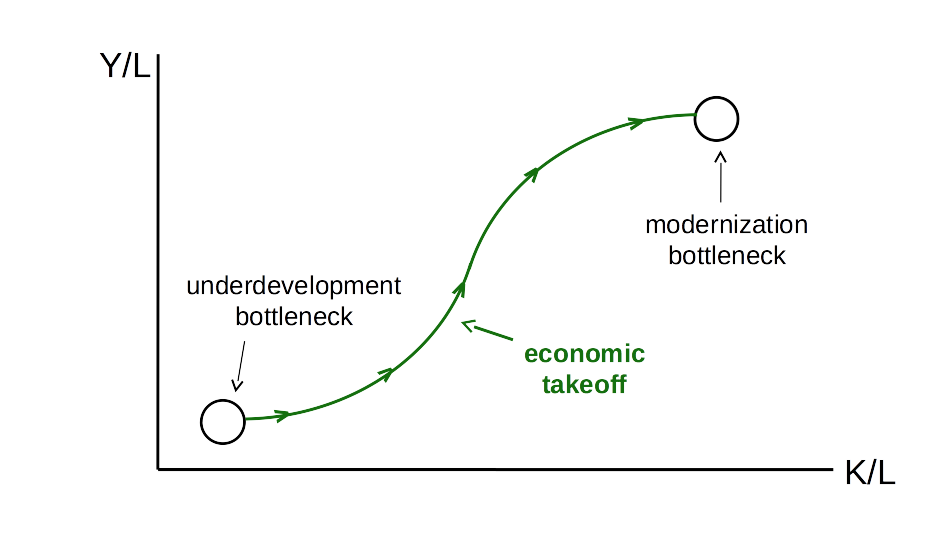
\includegraphics[scale=0.4]{figures/1}
	\caption{图示例}
\end{figure}

\lstinputlisting[caption={test.m}\label{aaa}]{codes/test.m}

	
\lstinputlisting[caption={test.m}\label{lt2}]{codes/test.m}

\ref*{lt1} \ref{lt2}

\section{参考文献例子}

参考文献。\ref{aaa}\cite{jls2003}\cite{Grisvard1985} 

{\bf 参考文献请务必用bibtex生成！！！}\cite{Agnelli2017,Ammari2007}


\chapter{结论}

Enjoy it.
\newline%%紧跟正文最后一个字符的不要删除！



%%%参考文献请务必用bibtex生成！！！
\bibliography{bib/ref.bib}	



\chapterx{致谢}

谢谢。本模板仅供内部使用，谢谢配合。



%\chapterx{个人简历}
%
%
\begin{resume}

\begin{resumesection}{基本情况}
某某某, 男/女, 某某省某某市/县人, 199？/200？ 年~？ 月出生.
\end{resumesection}

\begin{resumelist}{教育状况}
20XX 年~9 月至~20XX 年~7 月, 某某学校某某学院, 本科, 专业: XXXX。

20XX 年~9 月至~201XX年~7 月, 上海财经大学统计与管理学院, 硕士研究生, 专业: XXX。
\end{resumelist}
%
%\begin{resumelist}{工作经历}

%\end{resumelist}

\begin{resumesection}{研究兴趣}
XXXXX。
\end{resumesection}

\begin{resumesection}{联系方式}
E-mail: XXXXX@mail.shufe.edu.cn.
\end{resumesection}
%
\end{resume}




\end{document}
